
% Default to the notebook output style

    


% Inherit from the specified cell style.




    
\documentclass[11pt]{article}

    
    
    \usepackage[T1]{fontenc}
    % Nicer default font (+ math font) than Computer Modern for most use cases
    \usepackage{mathpazo}

    % Basic figure setup, for now with no caption control since it's done
    % automatically by Pandoc (which extracts ![](path) syntax from Markdown).
    \usepackage{graphicx}
    % We will generate all images so they have a width \maxwidth. This means
    % that they will get their normal width if they fit onto the page, but
    % are scaled down if they would overflow the margins.
    \makeatletter
    \def\maxwidth{\ifdim\Gin@nat@width>\linewidth\linewidth
    \else\Gin@nat@width\fi}
    \makeatother
    \let\Oldincludegraphics\includegraphics
    % Set max figure width to be 80% of text width, for now hardcoded.
    \renewcommand{\includegraphics}[1]{\Oldincludegraphics[width=.8\maxwidth]{#1}}
    % Ensure that by default, figures have no caption (until we provide a
    % proper Figure object with a Caption API and a way to capture that
    % in the conversion process - todo).
    \usepackage{caption}
    \DeclareCaptionLabelFormat{nolabel}{}
    \captionsetup{labelformat=nolabel}

    \usepackage{adjustbox} % Used to constrain images to a maximum size 
    \usepackage{xcolor} % Allow colors to be defined
    \usepackage{enumerate} % Needed for markdown enumerations to work
    \usepackage{geometry} % Used to adjust the document margins
    \usepackage{amsmath} % Equations
    \usepackage{amssymb} % Equations
    \usepackage{textcomp} % defines textquotesingle
    % Hack from http://tex.stackexchange.com/a/47451/13684:
    \AtBeginDocument{%
        \def\PYZsq{\textquotesingle}% Upright quotes in Pygmentized code
    }
    \usepackage{upquote} % Upright quotes for verbatim code
    \usepackage{eurosym} % defines \euro
    \usepackage[mathletters]{ucs} % Extended unicode (utf-8) support
    \usepackage[utf8x]{inputenc} % Allow utf-8 characters in the tex document
    \usepackage{fancyvrb} % verbatim replacement that allows latex
    \usepackage{grffile} % extends the file name processing of package graphics 
                         % to support a larger range 
    % The hyperref package gives us a pdf with properly built
    % internal navigation ('pdf bookmarks' for the table of contents,
    % internal cross-reference links, web links for URLs, etc.)
    \usepackage{hyperref}
    \usepackage{longtable} % longtable support required by pandoc >1.10
    \usepackage{booktabs}  % table support for pandoc > 1.12.2
    \usepackage[inline]{enumitem} % IRkernel/repr support (it uses the enumerate* environment)
    \usepackage[normalem]{ulem} % ulem is needed to support strikethroughs (\sout)
                                % normalem makes italics be italics, not underlines
    

    
    
    % Colors for the hyperref package
    \definecolor{urlcolor}{rgb}{0,.145,.698}
    \definecolor{linkcolor}{rgb}{.71,0.21,0.01}
    \definecolor{citecolor}{rgb}{.12,.54,.11}

    % ANSI colors
    \definecolor{ansi-black}{HTML}{3E424D}
    \definecolor{ansi-black-intense}{HTML}{282C36}
    \definecolor{ansi-red}{HTML}{E75C58}
    \definecolor{ansi-red-intense}{HTML}{B22B31}
    \definecolor{ansi-green}{HTML}{00A250}
    \definecolor{ansi-green-intense}{HTML}{007427}
    \definecolor{ansi-yellow}{HTML}{DDB62B}
    \definecolor{ansi-yellow-intense}{HTML}{B27D12}
    \definecolor{ansi-blue}{HTML}{208FFB}
    \definecolor{ansi-blue-intense}{HTML}{0065CA}
    \definecolor{ansi-magenta}{HTML}{D160C4}
    \definecolor{ansi-magenta-intense}{HTML}{A03196}
    \definecolor{ansi-cyan}{HTML}{60C6C8}
    \definecolor{ansi-cyan-intense}{HTML}{258F8F}
    \definecolor{ansi-white}{HTML}{C5C1B4}
    \definecolor{ansi-white-intense}{HTML}{A1A6B2}

    % commands and environments needed by pandoc snippets
    % extracted from the output of `pandoc -s`
    \providecommand{\tightlist}{%
      \setlength{\itemsep}{0pt}\setlength{\parskip}{0pt}}
    \DefineVerbatimEnvironment{Highlighting}{Verbatim}{commandchars=\\\{\}}
    % Add ',fontsize=\small' for more characters per line
    \newenvironment{Shaded}{}{}
    \newcommand{\KeywordTok}[1]{\textcolor[rgb]{0.00,0.44,0.13}{\textbf{{#1}}}}
    \newcommand{\DataTypeTok}[1]{\textcolor[rgb]{0.56,0.13,0.00}{{#1}}}
    \newcommand{\DecValTok}[1]{\textcolor[rgb]{0.25,0.63,0.44}{{#1}}}
    \newcommand{\BaseNTok}[1]{\textcolor[rgb]{0.25,0.63,0.44}{{#1}}}
    \newcommand{\FloatTok}[1]{\textcolor[rgb]{0.25,0.63,0.44}{{#1}}}
    \newcommand{\CharTok}[1]{\textcolor[rgb]{0.25,0.44,0.63}{{#1}}}
    \newcommand{\StringTok}[1]{\textcolor[rgb]{0.25,0.44,0.63}{{#1}}}
    \newcommand{\CommentTok}[1]{\textcolor[rgb]{0.38,0.63,0.69}{\textit{{#1}}}}
    \newcommand{\OtherTok}[1]{\textcolor[rgb]{0.00,0.44,0.13}{{#1}}}
    \newcommand{\AlertTok}[1]{\textcolor[rgb]{1.00,0.00,0.00}{\textbf{{#1}}}}
    \newcommand{\FunctionTok}[1]{\textcolor[rgb]{0.02,0.16,0.49}{{#1}}}
    \newcommand{\RegionMarkerTok}[1]{{#1}}
    \newcommand{\ErrorTok}[1]{\textcolor[rgb]{1.00,0.00,0.00}{\textbf{{#1}}}}
    \newcommand{\NormalTok}[1]{{#1}}
    
    % Additional commands for more recent versions of Pandoc
    \newcommand{\ConstantTok}[1]{\textcolor[rgb]{0.53,0.00,0.00}{{#1}}}
    \newcommand{\SpecialCharTok}[1]{\textcolor[rgb]{0.25,0.44,0.63}{{#1}}}
    \newcommand{\VerbatimStringTok}[1]{\textcolor[rgb]{0.25,0.44,0.63}{{#1}}}
    \newcommand{\SpecialStringTok}[1]{\textcolor[rgb]{0.73,0.40,0.53}{{#1}}}
    \newcommand{\ImportTok}[1]{{#1}}
    \newcommand{\DocumentationTok}[1]{\textcolor[rgb]{0.73,0.13,0.13}{\textit{{#1}}}}
    \newcommand{\AnnotationTok}[1]{\textcolor[rgb]{0.38,0.63,0.69}{\textbf{\textit{{#1}}}}}
    \newcommand{\CommentVarTok}[1]{\textcolor[rgb]{0.38,0.63,0.69}{\textbf{\textit{{#1}}}}}
    \newcommand{\VariableTok}[1]{\textcolor[rgb]{0.10,0.09,0.49}{{#1}}}
    \newcommand{\ControlFlowTok}[1]{\textcolor[rgb]{0.00,0.44,0.13}{\textbf{{#1}}}}
    \newcommand{\OperatorTok}[1]{\textcolor[rgb]{0.40,0.40,0.40}{{#1}}}
    \newcommand{\BuiltInTok}[1]{{#1}}
    \newcommand{\ExtensionTok}[1]{{#1}}
    \newcommand{\PreprocessorTok}[1]{\textcolor[rgb]{0.74,0.48,0.00}{{#1}}}
    \newcommand{\AttributeTok}[1]{\textcolor[rgb]{0.49,0.56,0.16}{{#1}}}
    \newcommand{\InformationTok}[1]{\textcolor[rgb]{0.38,0.63,0.69}{\textbf{\textit{{#1}}}}}
    \newcommand{\WarningTok}[1]{\textcolor[rgb]{0.38,0.63,0.69}{\textbf{\textit{{#1}}}}}
    
    
    % Define a nice break command that doesn't care if a line doesn't already
    % exist.
    \def\br{\hspace*{\fill} \\* }
    % Math Jax compatability definitions
    \def\gt{>}
    \def\lt{<}
    % Document parameters
    \title{chapter\_03}
    
    
    

    % Pygments definitions
    
\makeatletter
\def\PY@reset{\let\PY@it=\relax \let\PY@bf=\relax%
    \let\PY@ul=\relax \let\PY@tc=\relax%
    \let\PY@bc=\relax \let\PY@ff=\relax}
\def\PY@tok#1{\csname PY@tok@#1\endcsname}
\def\PY@toks#1+{\ifx\relax#1\empty\else%
    \PY@tok{#1}\expandafter\PY@toks\fi}
\def\PY@do#1{\PY@bc{\PY@tc{\PY@ul{%
    \PY@it{\PY@bf{\PY@ff{#1}}}}}}}
\def\PY#1#2{\PY@reset\PY@toks#1+\relax+\PY@do{#2}}

\expandafter\def\csname PY@tok@w\endcsname{\def\PY@tc##1{\textcolor[rgb]{0.73,0.73,0.73}{##1}}}
\expandafter\def\csname PY@tok@c\endcsname{\let\PY@it=\textit\def\PY@tc##1{\textcolor[rgb]{0.25,0.50,0.50}{##1}}}
\expandafter\def\csname PY@tok@cp\endcsname{\def\PY@tc##1{\textcolor[rgb]{0.74,0.48,0.00}{##1}}}
\expandafter\def\csname PY@tok@k\endcsname{\let\PY@bf=\textbf\def\PY@tc##1{\textcolor[rgb]{0.00,0.50,0.00}{##1}}}
\expandafter\def\csname PY@tok@kp\endcsname{\def\PY@tc##1{\textcolor[rgb]{0.00,0.50,0.00}{##1}}}
\expandafter\def\csname PY@tok@kt\endcsname{\def\PY@tc##1{\textcolor[rgb]{0.69,0.00,0.25}{##1}}}
\expandafter\def\csname PY@tok@o\endcsname{\def\PY@tc##1{\textcolor[rgb]{0.40,0.40,0.40}{##1}}}
\expandafter\def\csname PY@tok@ow\endcsname{\let\PY@bf=\textbf\def\PY@tc##1{\textcolor[rgb]{0.67,0.13,1.00}{##1}}}
\expandafter\def\csname PY@tok@nb\endcsname{\def\PY@tc##1{\textcolor[rgb]{0.00,0.50,0.00}{##1}}}
\expandafter\def\csname PY@tok@nf\endcsname{\def\PY@tc##1{\textcolor[rgb]{0.00,0.00,1.00}{##1}}}
\expandafter\def\csname PY@tok@nc\endcsname{\let\PY@bf=\textbf\def\PY@tc##1{\textcolor[rgb]{0.00,0.00,1.00}{##1}}}
\expandafter\def\csname PY@tok@nn\endcsname{\let\PY@bf=\textbf\def\PY@tc##1{\textcolor[rgb]{0.00,0.00,1.00}{##1}}}
\expandafter\def\csname PY@tok@ne\endcsname{\let\PY@bf=\textbf\def\PY@tc##1{\textcolor[rgb]{0.82,0.25,0.23}{##1}}}
\expandafter\def\csname PY@tok@nv\endcsname{\def\PY@tc##1{\textcolor[rgb]{0.10,0.09,0.49}{##1}}}
\expandafter\def\csname PY@tok@no\endcsname{\def\PY@tc##1{\textcolor[rgb]{0.53,0.00,0.00}{##1}}}
\expandafter\def\csname PY@tok@nl\endcsname{\def\PY@tc##1{\textcolor[rgb]{0.63,0.63,0.00}{##1}}}
\expandafter\def\csname PY@tok@ni\endcsname{\let\PY@bf=\textbf\def\PY@tc##1{\textcolor[rgb]{0.60,0.60,0.60}{##1}}}
\expandafter\def\csname PY@tok@na\endcsname{\def\PY@tc##1{\textcolor[rgb]{0.49,0.56,0.16}{##1}}}
\expandafter\def\csname PY@tok@nt\endcsname{\let\PY@bf=\textbf\def\PY@tc##1{\textcolor[rgb]{0.00,0.50,0.00}{##1}}}
\expandafter\def\csname PY@tok@nd\endcsname{\def\PY@tc##1{\textcolor[rgb]{0.67,0.13,1.00}{##1}}}
\expandafter\def\csname PY@tok@s\endcsname{\def\PY@tc##1{\textcolor[rgb]{0.73,0.13,0.13}{##1}}}
\expandafter\def\csname PY@tok@sd\endcsname{\let\PY@it=\textit\def\PY@tc##1{\textcolor[rgb]{0.73,0.13,0.13}{##1}}}
\expandafter\def\csname PY@tok@si\endcsname{\let\PY@bf=\textbf\def\PY@tc##1{\textcolor[rgb]{0.73,0.40,0.53}{##1}}}
\expandafter\def\csname PY@tok@se\endcsname{\let\PY@bf=\textbf\def\PY@tc##1{\textcolor[rgb]{0.73,0.40,0.13}{##1}}}
\expandafter\def\csname PY@tok@sr\endcsname{\def\PY@tc##1{\textcolor[rgb]{0.73,0.40,0.53}{##1}}}
\expandafter\def\csname PY@tok@ss\endcsname{\def\PY@tc##1{\textcolor[rgb]{0.10,0.09,0.49}{##1}}}
\expandafter\def\csname PY@tok@sx\endcsname{\def\PY@tc##1{\textcolor[rgb]{0.00,0.50,0.00}{##1}}}
\expandafter\def\csname PY@tok@m\endcsname{\def\PY@tc##1{\textcolor[rgb]{0.40,0.40,0.40}{##1}}}
\expandafter\def\csname PY@tok@gh\endcsname{\let\PY@bf=\textbf\def\PY@tc##1{\textcolor[rgb]{0.00,0.00,0.50}{##1}}}
\expandafter\def\csname PY@tok@gu\endcsname{\let\PY@bf=\textbf\def\PY@tc##1{\textcolor[rgb]{0.50,0.00,0.50}{##1}}}
\expandafter\def\csname PY@tok@gd\endcsname{\def\PY@tc##1{\textcolor[rgb]{0.63,0.00,0.00}{##1}}}
\expandafter\def\csname PY@tok@gi\endcsname{\def\PY@tc##1{\textcolor[rgb]{0.00,0.63,0.00}{##1}}}
\expandafter\def\csname PY@tok@gr\endcsname{\def\PY@tc##1{\textcolor[rgb]{1.00,0.00,0.00}{##1}}}
\expandafter\def\csname PY@tok@ge\endcsname{\let\PY@it=\textit}
\expandafter\def\csname PY@tok@gs\endcsname{\let\PY@bf=\textbf}
\expandafter\def\csname PY@tok@gp\endcsname{\let\PY@bf=\textbf\def\PY@tc##1{\textcolor[rgb]{0.00,0.00,0.50}{##1}}}
\expandafter\def\csname PY@tok@go\endcsname{\def\PY@tc##1{\textcolor[rgb]{0.53,0.53,0.53}{##1}}}
\expandafter\def\csname PY@tok@gt\endcsname{\def\PY@tc##1{\textcolor[rgb]{0.00,0.27,0.87}{##1}}}
\expandafter\def\csname PY@tok@err\endcsname{\def\PY@bc##1{\setlength{\fboxsep}{0pt}\fcolorbox[rgb]{1.00,0.00,0.00}{1,1,1}{\strut ##1}}}
\expandafter\def\csname PY@tok@kc\endcsname{\let\PY@bf=\textbf\def\PY@tc##1{\textcolor[rgb]{0.00,0.50,0.00}{##1}}}
\expandafter\def\csname PY@tok@kd\endcsname{\let\PY@bf=\textbf\def\PY@tc##1{\textcolor[rgb]{0.00,0.50,0.00}{##1}}}
\expandafter\def\csname PY@tok@kn\endcsname{\let\PY@bf=\textbf\def\PY@tc##1{\textcolor[rgb]{0.00,0.50,0.00}{##1}}}
\expandafter\def\csname PY@tok@kr\endcsname{\let\PY@bf=\textbf\def\PY@tc##1{\textcolor[rgb]{0.00,0.50,0.00}{##1}}}
\expandafter\def\csname PY@tok@bp\endcsname{\def\PY@tc##1{\textcolor[rgb]{0.00,0.50,0.00}{##1}}}
\expandafter\def\csname PY@tok@fm\endcsname{\def\PY@tc##1{\textcolor[rgb]{0.00,0.00,1.00}{##1}}}
\expandafter\def\csname PY@tok@vc\endcsname{\def\PY@tc##1{\textcolor[rgb]{0.10,0.09,0.49}{##1}}}
\expandafter\def\csname PY@tok@vg\endcsname{\def\PY@tc##1{\textcolor[rgb]{0.10,0.09,0.49}{##1}}}
\expandafter\def\csname PY@tok@vi\endcsname{\def\PY@tc##1{\textcolor[rgb]{0.10,0.09,0.49}{##1}}}
\expandafter\def\csname PY@tok@vm\endcsname{\def\PY@tc##1{\textcolor[rgb]{0.10,0.09,0.49}{##1}}}
\expandafter\def\csname PY@tok@sa\endcsname{\def\PY@tc##1{\textcolor[rgb]{0.73,0.13,0.13}{##1}}}
\expandafter\def\csname PY@tok@sb\endcsname{\def\PY@tc##1{\textcolor[rgb]{0.73,0.13,0.13}{##1}}}
\expandafter\def\csname PY@tok@sc\endcsname{\def\PY@tc##1{\textcolor[rgb]{0.73,0.13,0.13}{##1}}}
\expandafter\def\csname PY@tok@dl\endcsname{\def\PY@tc##1{\textcolor[rgb]{0.73,0.13,0.13}{##1}}}
\expandafter\def\csname PY@tok@s2\endcsname{\def\PY@tc##1{\textcolor[rgb]{0.73,0.13,0.13}{##1}}}
\expandafter\def\csname PY@tok@sh\endcsname{\def\PY@tc##1{\textcolor[rgb]{0.73,0.13,0.13}{##1}}}
\expandafter\def\csname PY@tok@s1\endcsname{\def\PY@tc##1{\textcolor[rgb]{0.73,0.13,0.13}{##1}}}
\expandafter\def\csname PY@tok@mb\endcsname{\def\PY@tc##1{\textcolor[rgb]{0.40,0.40,0.40}{##1}}}
\expandafter\def\csname PY@tok@mf\endcsname{\def\PY@tc##1{\textcolor[rgb]{0.40,0.40,0.40}{##1}}}
\expandafter\def\csname PY@tok@mh\endcsname{\def\PY@tc##1{\textcolor[rgb]{0.40,0.40,0.40}{##1}}}
\expandafter\def\csname PY@tok@mi\endcsname{\def\PY@tc##1{\textcolor[rgb]{0.40,0.40,0.40}{##1}}}
\expandafter\def\csname PY@tok@il\endcsname{\def\PY@tc##1{\textcolor[rgb]{0.40,0.40,0.40}{##1}}}
\expandafter\def\csname PY@tok@mo\endcsname{\def\PY@tc##1{\textcolor[rgb]{0.40,0.40,0.40}{##1}}}
\expandafter\def\csname PY@tok@ch\endcsname{\let\PY@it=\textit\def\PY@tc##1{\textcolor[rgb]{0.25,0.50,0.50}{##1}}}
\expandafter\def\csname PY@tok@cm\endcsname{\let\PY@it=\textit\def\PY@tc##1{\textcolor[rgb]{0.25,0.50,0.50}{##1}}}
\expandafter\def\csname PY@tok@cpf\endcsname{\let\PY@it=\textit\def\PY@tc##1{\textcolor[rgb]{0.25,0.50,0.50}{##1}}}
\expandafter\def\csname PY@tok@c1\endcsname{\let\PY@it=\textit\def\PY@tc##1{\textcolor[rgb]{0.25,0.50,0.50}{##1}}}
\expandafter\def\csname PY@tok@cs\endcsname{\let\PY@it=\textit\def\PY@tc##1{\textcolor[rgb]{0.25,0.50,0.50}{##1}}}

\def\PYZbs{\char`\\}
\def\PYZus{\char`\_}
\def\PYZob{\char`\{}
\def\PYZcb{\char`\}}
\def\PYZca{\char`\^}
\def\PYZam{\char`\&}
\def\PYZlt{\char`\<}
\def\PYZgt{\char`\>}
\def\PYZsh{\char`\#}
\def\PYZpc{\char`\%}
\def\PYZdl{\char`\$}
\def\PYZhy{\char`\-}
\def\PYZsq{\char`\'}
\def\PYZdq{\char`\"}
\def\PYZti{\char`\~}
% for compatibility with earlier versions
\def\PYZat{@}
\def\PYZlb{[}
\def\PYZrb{]}
\makeatother


    % Exact colors from NB
    \definecolor{incolor}{rgb}{0.0, 0.0, 0.5}
    \definecolor{outcolor}{rgb}{0.545, 0.0, 0.0}



    
    % Prevent overflowing lines due to hard-to-break entities
    \sloppy 
    % Setup hyperref package
    \hypersetup{
      breaklinks=true,  % so long urls are correctly broken across lines
      colorlinks=true,
      urlcolor=urlcolor,
      linkcolor=linkcolor,
      citecolor=citecolor,
      }
    % Slightly bigger margins than the latex defaults
    
    \geometry{verbose,tmargin=1in,bmargin=1in,lmargin=1in,rmargin=1in}
    
    

    \begin{document}
    
    
    \maketitle
    
    

    
    \section{Training a perceptron; First steps with
scikit-learn.}\label{training-a-perceptron-first-steps-with-scikit-learn.}

\begin{itemize}
\tightlist
\item
  We will only use the 2 features from the Iris dataset for
  visualisation purposes.
\item
  We will assign the petal length and the petal width of the 150 flower
  samples to the feature matrix \texttt{X}.
\item
  The corresponding class labels of the flower species are assigned to
  the vector \texttt{y}.
\end{itemize}

    \begin{Verbatim}[commandchars=\\\{\}]
{\color{incolor}In [{\color{incolor}1}]:} \PY{k+kn}{from} \PY{n+nn}{sklearn} \PY{k}{import} \PY{n}{datasets}
        \PY{k+kn}{import} \PY{n+nn}{numpy} \PY{k}{as} \PY{n+nn}{np}
        
        \PY{n}{iris} \PY{o}{=} \PY{n}{datasets}\PY{o}{.}\PY{n}{load\PYZus{}iris}\PY{p}{(}\PY{p}{)}
        \PY{n}{X} \PY{o}{=} \PY{n}{iris}\PY{o}{.}\PY{n}{data}\PY{p}{[}\PY{p}{:}\PY{p}{,} \PY{p}{[}\PY{l+m+mi}{2}\PY{p}{,} \PY{l+m+mi}{3}\PY{p}{]}\PY{p}{]}  \PY{c+c1}{\PYZsh{} we are only interested in the petal length and the petal width.}
        \PY{n}{y} \PY{o}{=} \PY{n}{iris}\PY{o}{.}\PY{n}{target}
        \PY{n+nb}{print}\PY{p}{(}\PY{l+s+s1}{\PYZsq{}}\PY{l+s+s1}{Class labels: }\PY{l+s+si}{\PYZob{}\PYZcb{}}\PY{l+s+s1}{.}\PY{l+s+s1}{\PYZsq{}}\PY{o}{.}\PY{n}{format}\PY{p}{(}\PY{n}{np}\PY{o}{.}\PY{n}{unique}\PY{p}{(}\PY{n}{y}\PY{p}{)}\PY{p}{)}\PY{p}{)}
\end{Verbatim}


    \begin{Verbatim}[commandchars=\\\{\}]
Class labels: [0 1 2].

    \end{Verbatim}

    \subsection{Evaluation}\label{evaluation}

In order to evaluate how well a trained model performs on unseens data,
we will further split the dataset into separate training and test
datasets.

In the following we randomply split the X and y arrays into 30 percent
test data (45 samples) and 70 percent training data (105 samples).

    \begin{Verbatim}[commandchars=\\\{\}]
{\color{incolor}In [{\color{incolor}2}]:} \PY{k+kn}{from} \PY{n+nn}{sklearn}\PY{n+nn}{.}\PY{n+nn}{model\PYZus{}selection} \PY{k}{import} \PY{n}{train\PYZus{}test\PYZus{}split}
        \PY{n}{X\PYZus{}train}\PY{p}{,} \PY{n}{X\PYZus{}test}\PY{p}{,} \PY{n}{y\PYZus{}train}\PY{p}{,} \PY{n}{y\PYZus{}test} \PY{o}{=} \PY{n}{train\PYZus{}test\PYZus{}split}\PY{p}{(}\PY{n}{X}\PY{p}{,} \PY{n}{y}\PY{p}{,} \PY{n}{test\PYZus{}size}\PY{o}{=}\PY{l+m+mf}{0.3}\PY{p}{,}
                                                            \PY{n}{random\PYZus{}state}\PY{o}{=}\PY{l+m+mi}{1}\PY{p}{,} \PY{n}{stratify}\PY{o}{=}\PY{n}{y}\PY{p}{)}
\end{Verbatim}


    \subsubsection{Comments on the above
code}\label{comments-on-the-above-code}

\begin{itemize}
\tightlist
\item
  \texttt{train\_test\_split} function already shuffles the training
  sets internally before splitting.
\item
  Stratification means that the \texttt{train\_test\_split} method
  returns training and test subsets that have the same proportions of
  class labels as the input dataset. We can use NumPy's
  \texttt{bincount} function, which counts the number of occurrences of
  each value in an array.
\end{itemize}

    \begin{Verbatim}[commandchars=\\\{\}]
{\color{incolor}In [{\color{incolor}3}]:} \PY{n+nb}{print}\PY{p}{(}\PY{l+s+s1}{\PYZsq{}}\PY{l+s+s1}{Label counts in y: }\PY{l+s+si}{\PYZob{}\PYZcb{}}\PY{l+s+s1}{\PYZsq{}}\PY{o}{.}\PY{n}{format}\PY{p}{(}\PY{n}{np}\PY{o}{.}\PY{n}{bincount}\PY{p}{(}\PY{n}{y}\PY{p}{)}\PY{p}{)}\PY{p}{)}
        \PY{n+nb}{print}\PY{p}{(}\PY{l+s+s1}{\PYZsq{}}\PY{l+s+s1}{Label counts in y\PYZus{}train: }\PY{l+s+si}{\PYZob{}\PYZcb{}}\PY{l+s+s1}{\PYZsq{}}\PY{o}{.}\PY{n}{format}\PY{p}{(}\PY{n}{np}\PY{o}{.}\PY{n}{bincount}\PY{p}{(}\PY{n}{y\PYZus{}train}\PY{p}{)}\PY{p}{)}\PY{p}{)}
        \PY{n+nb}{print}\PY{p}{(}\PY{l+s+s1}{\PYZsq{}}\PY{l+s+s1}{Label counts in t\PYZus{}test: }\PY{l+s+si}{\PYZob{}\PYZcb{}}\PY{l+s+s1}{\PYZsq{}}\PY{o}{.}\PY{n}{format}\PY{p}{(}\PY{n}{np}\PY{o}{.}\PY{n}{bincount}\PY{p}{(}\PY{n}{y\PYZus{}test}\PY{p}{)}\PY{p}{)}\PY{p}{)}
\end{Verbatim}


    \begin{Verbatim}[commandchars=\\\{\}]
Label counts in y: [50 50 50]
Label counts in y\_train: [35 35 35]
Label counts in t\_test: [15 15 15]

    \end{Verbatim}

    \subsection{Standardisation}\label{standardisation}

Up next, we standardise the features using the \texttt{StandardScaler}
class from scikit-learn's \texttt{preprocessing} module.

    \begin{Verbatim}[commandchars=\\\{\}]
{\color{incolor}In [{\color{incolor}4}]:} \PY{k+kn}{from} \PY{n+nn}{sklearn}\PY{n+nn}{.}\PY{n+nn}{preprocessing} \PY{k}{import} \PY{n}{StandardScaler}
        \PY{n}{sc} \PY{o}{=} \PY{n}{StandardScaler}\PY{p}{(}\PY{p}{)}
        \PY{n}{sc}\PY{o}{.}\PY{n}{fit}\PY{p}{(}\PY{n}{X\PYZus{}train}\PY{p}{)}
        
        \PY{n}{X\PYZus{}train\PYZus{}std} \PY{o}{=} \PY{n}{sc}\PY{o}{.}\PY{n}{transform}\PY{p}{(}\PY{n}{X\PYZus{}train}\PY{p}{)}
        \PY{n}{X\PYZus{}test\PYZus{}std} \PY{o}{=} \PY{n}{sc}\PY{o}{.}\PY{n}{transform}\PY{p}{(}\PY{n}{X\PYZus{}test}\PY{p}{)}
\end{Verbatim}


    \subsubsection{Comments on the above
code}\label{comments-on-the-above-code}

\begin{itemize}
\tightlist
\item
  Using the \texttt{fit} method, \texttt{StandardScaler} estimated the
  parameters \(\mu\) and \(\sigma\) for each feature dimension from the
  training data.
\item
  By calling the transform method, we then standardise the training data
  using those estimated parameters \(\mu\) and \(\sigma\).
\end{itemize}

    \subsection{One-versus-Rest (OvR)}\label{one-versus-rest-ovr}

\begin{itemize}
\tightlist
\item
  scikit-learn already supports multiclass classification by default via
  the OvR method.
\item
  This allows us to feed the 3 flower classes to the perceptron all at
  once.
\end{itemize}

The code is as follows:

    \begin{Verbatim}[commandchars=\\\{\}]
{\color{incolor}In [{\color{incolor}5}]:} \PY{k+kn}{from} \PY{n+nn}{sklearn}\PY{n+nn}{.}\PY{n+nn}{linear\PYZus{}model} \PY{k}{import} \PY{n}{Perceptron}
        
        \PY{n}{ppn} \PY{o}{=} \PY{n}{Perceptron}\PY{p}{(}\PY{n}{max\PYZus{}iter}\PY{o}{=}\PY{l+m+mi}{40}\PY{p}{,} \PY{n}{eta0}\PY{o}{=}\PY{l+m+mf}{0.1}\PY{p}{,} \PY{n}{random\PYZus{}state}\PY{o}{=}\PY{l+m+mi}{1}\PY{p}{)}
        \PY{n}{ppn}\PY{o}{.}\PY{n}{fit}\PY{p}{(}\PY{n}{X\PYZus{}train\PYZus{}std}\PY{p}{,} \PY{n}{y\PYZus{}train}\PY{p}{)}
\end{Verbatim}


\begin{Verbatim}[commandchars=\\\{\}]
{\color{outcolor}Out[{\color{outcolor}5}]:} Perceptron(alpha=0.0001, class\_weight=None, eta0=0.1, fit\_intercept=True,
              max\_iter=40, n\_iter=None, n\_jobs=1, penalty=None, random\_state=1,
              shuffle=True, tol=None, verbose=0, warm\_start=False)
\end{Verbatim}
            
    \subsection{\texorpdfstring{Making predictions via the \texttt{predict}
method:}{Making predictions via the predict method:}}\label{making-predictions-via-the-predict-method}

    \begin{Verbatim}[commandchars=\\\{\}]
{\color{incolor}In [{\color{incolor}6}]:} \PY{n}{y\PYZus{}pred} \PY{o}{=} \PY{n}{ppn}\PY{o}{.}\PY{n}{predict}\PY{p}{(}\PY{n}{X\PYZus{}test\PYZus{}std}\PY{p}{)}
        \PY{n+nb}{print}\PY{p}{(}\PY{l+s+s1}{\PYZsq{}}\PY{l+s+s1}{Misclassified samples: }\PY{l+s+si}{\PYZob{}\PYZcb{}}\PY{l+s+s1}{\PYZsq{}}\PY{o}{.}\PY{n}{format}\PY{p}{(}\PY{p}{(}\PY{n}{y\PYZus{}test} \PY{o}{!=} \PY{n}{y\PYZus{}pred}\PY{p}{)}\PY{o}{.}\PY{n}{sum}\PY{p}{(}\PY{p}{)}\PY{p}{)}\PY{p}{)}
\end{Verbatim}


    \begin{Verbatim}[commandchars=\\\{\}]
Misclassified samples: 3

    \end{Verbatim}

    \subsection{Performance metrics}\label{performance-metrics}

The scikit-learn library also implements a large variety of different
performance metrics that are available via the \texttt{metrics} module.

For example, we can calculate the classification accuracy of the
perceptron on the test set as follows:

    \begin{Verbatim}[commandchars=\\\{\}]
{\color{incolor}In [{\color{incolor}7}]:} \PY{k+kn}{from} \PY{n+nn}{sklearn}\PY{n+nn}{.}\PY{n+nn}{metrics} \PY{k}{import} \PY{n}{accuracy\PYZus{}score}
        \PY{n+nb}{print}\PY{p}{(}\PY{l+s+s1}{\PYZsq{}}\PY{l+s+s1}{Accuracy: }\PY{l+s+si}{\PYZob{}0:.2f\PYZcb{}}\PY{l+s+s1}{\PYZsq{}}\PY{o}{.}\PY{n}{format}\PY{p}{(}\PY{n}{accuracy\PYZus{}score}\PY{p}{(}\PY{n}{y\PYZus{}test}\PY{p}{,} \PY{n}{y\PYZus{}pred}\PY{p}{)}\PY{p}{)}\PY{p}{)}
\end{Verbatim}


    \begin{Verbatim}[commandchars=\\\{\}]
Accuracy: 0.93

    \end{Verbatim}

    Alternatively, each classifier in scikit-learn has a \texttt{score}
method, which computes a classifier's prediction accuracy by combining
the \texttt{predict} call with \texttt{accuracy\_score} as shown here:

    \begin{Verbatim}[commandchars=\\\{\}]
{\color{incolor}In [{\color{incolor}8}]:} \PY{n+nb}{print}\PY{p}{(}\PY{l+s+s1}{\PYZsq{}}\PY{l+s+s1}{Accuracy: }\PY{l+s+si}{\PYZob{}0:.2f\PYZcb{}}\PY{l+s+s1}{\PYZsq{}}\PY{o}{.}\PY{n}{format}\PY{p}{(}\PY{n}{ppn}\PY{o}{.}\PY{n}{score}\PY{p}{(}\PY{n}{X\PYZus{}test\PYZus{}std}\PY{p}{,} \PY{n}{y\PYZus{}test}\PY{p}{)}\PY{p}{)}\PY{p}{)}
\end{Verbatim}


    \begin{Verbatim}[commandchars=\\\{\}]
Accuracy: 0.93

    \end{Verbatim}

    \subsection{Decision regions}\label{decision-regions}

Finally we get to use our \texttt{plot\_decision\_regions} function from
Chapter 2 to plot the decision regions or our newly trained perceptron
model and visualise how well it separates the different flower samples.
However, let's add a small modification to highlight the samples from
the test dataset via small circles:

    \begin{Verbatim}[commandchars=\\\{\}]
{\color{incolor}In [{\color{incolor}9}]:} \PY{k+kn}{from} \PY{n+nn}{matplotlib}\PY{n+nn}{.}\PY{n+nn}{colors} \PY{k}{import} \PY{n}{ListedColormap}
        \PY{k+kn}{import} \PY{n+nn}{matplotlib}\PY{n+nn}{.}\PY{n+nn}{pyplot} \PY{k}{as} \PY{n+nn}{plt}
        
        \PY{k}{def} \PY{n+nf}{plot\PYZus{}decision\PYZus{}regions}\PY{p}{(}\PY{n}{X}\PY{p}{,} \PY{n}{y}\PY{p}{,} \PY{n}{classifier}\PY{p}{,} \PY{n}{test\PYZus{}idx}\PY{o}{=}\PY{k+kc}{None}\PY{p}{,} \PY{n}{resolution}\PY{o}{=}\PY{l+m+mf}{0.02}\PY{p}{)}\PY{p}{:}
            \PY{c+c1}{\PYZsh{} setup the marker generator and color map}
            \PY{n}{markers} \PY{o}{=} \PY{p}{(}\PY{l+s+s1}{\PYZsq{}}\PY{l+s+s1}{s}\PY{l+s+s1}{\PYZsq{}}\PY{p}{,} \PY{l+s+s1}{\PYZsq{}}\PY{l+s+s1}{x}\PY{l+s+s1}{\PYZsq{}}\PY{p}{,} \PY{l+s+s1}{\PYZsq{}}\PY{l+s+s1}{o}\PY{l+s+s1}{\PYZsq{}}\PY{p}{,} \PY{l+s+s1}{\PYZsq{}}\PY{l+s+s1}{\PYZca{}}\PY{l+s+s1}{\PYZsq{}}\PY{p}{,} \PY{l+s+s1}{\PYZsq{}}\PY{l+s+s1}{v}\PY{l+s+s1}{\PYZsq{}}\PY{p}{)}
            \PY{n}{colors} \PY{o}{=} \PY{p}{(}\PY{l+s+s1}{\PYZsq{}}\PY{l+s+s1}{red}\PY{l+s+s1}{\PYZsq{}}\PY{p}{,} \PY{l+s+s1}{\PYZsq{}}\PY{l+s+s1}{blue}\PY{l+s+s1}{\PYZsq{}}\PY{p}{,} \PY{l+s+s1}{\PYZsq{}}\PY{l+s+s1}{lightgreen}\PY{l+s+s1}{\PYZsq{}}\PY{p}{,} \PY{l+s+s1}{\PYZsq{}}\PY{l+s+s1}{gray}\PY{l+s+s1}{\PYZsq{}}\PY{p}{,} \PY{l+s+s1}{\PYZsq{}}\PY{l+s+s1}{cyan}\PY{l+s+s1}{\PYZsq{}}\PY{p}{)}
            \PY{n}{cmap} \PY{o}{=} \PY{n}{ListedColormap}\PY{p}{(}\PY{n}{colors}\PY{p}{[}\PY{p}{:}\PY{n+nb}{len}\PY{p}{(}\PY{n}{np}\PY{o}{.}\PY{n}{unique}\PY{p}{(}\PY{n}{y}\PY{p}{)}\PY{p}{)}\PY{p}{]}\PY{p}{)}
            
            \PY{c+c1}{\PYZsh{} plot the decision surfaces}
            \PY{n}{x1\PYZus{}min}\PY{p}{,} \PY{n}{x1\PYZus{}max} \PY{o}{=} \PY{n}{X}\PY{p}{[}\PY{p}{:}\PY{p}{,} \PY{l+m+mi}{0}\PY{p}{]}\PY{o}{.}\PY{n}{min}\PY{p}{(}\PY{p}{)} \PY{o}{\PYZhy{}} \PY{l+m+mi}{1}\PY{p}{,} \PY{n}{X}\PY{p}{[}\PY{p}{:}\PY{p}{,} \PY{l+m+mi}{0}\PY{p}{]}\PY{o}{.}\PY{n}{max}\PY{p}{(}\PY{p}{)} \PY{o}{+} \PY{l+m+mi}{1}
            \PY{n}{x2\PYZus{}min}\PY{p}{,} \PY{n}{x2\PYZus{}max} \PY{o}{=} \PY{n}{X}\PY{p}{[}\PY{p}{:}\PY{p}{,} \PY{l+m+mi}{1}\PY{p}{]}\PY{o}{.}\PY{n}{min}\PY{p}{(}\PY{p}{)} \PY{o}{\PYZhy{}} \PY{l+m+mi}{1}\PY{p}{,} \PY{n}{X}\PY{p}{[}\PY{p}{:}\PY{p}{,} \PY{l+m+mi}{1}\PY{p}{]}\PY{o}{.}\PY{n}{max}\PY{p}{(}\PY{p}{)} \PY{o}{+} \PY{l+m+mi}{1}
            \PY{n}{xx1}\PY{p}{,} \PY{n}{xx2} \PY{o}{=} \PY{n}{np}\PY{o}{.}\PY{n}{meshgrid}\PY{p}{(}\PY{n}{np}\PY{o}{.}\PY{n}{arange}\PY{p}{(}\PY{n}{x1\PYZus{}min}\PY{p}{,} \PY{n}{x1\PYZus{}max}\PY{p}{,} \PY{n}{resolution}\PY{p}{)}\PY{p}{,}
                                   \PY{n}{np}\PY{o}{.}\PY{n}{arange}\PY{p}{(}\PY{n}{x2\PYZus{}min}\PY{p}{,} \PY{n}{x2\PYZus{}max}\PY{p}{,} \PY{n}{resolution}\PY{p}{)}\PY{p}{)}
            
            \PY{n}{Z} \PY{o}{=} \PY{n}{classifier}\PY{o}{.}\PY{n}{predict}\PY{p}{(}\PY{n}{np}\PY{o}{.}\PY{n}{array}\PY{p}{(}\PY{p}{[}\PY{n}{xx1}\PY{o}{.}\PY{n}{ravel}\PY{p}{(}\PY{p}{)}\PY{p}{,} \PY{n}{xx2}\PY{o}{.}\PY{n}{ravel}\PY{p}{(}\PY{p}{)}\PY{p}{]}\PY{p}{)}\PY{o}{.}\PY{n}{T}\PY{p}{)}
            \PY{n}{Z} \PY{o}{=} \PY{n}{Z}\PY{o}{.}\PY{n}{reshape}\PY{p}{(}\PY{n}{xx1}\PY{o}{.}\PY{n}{shape}\PY{p}{)}
            \PY{n}{plt}\PY{o}{.}\PY{n}{contourf}\PY{p}{(}\PY{n}{xx1}\PY{p}{,} \PY{n}{xx2}\PY{p}{,} \PY{n}{Z}\PY{p}{,} \PY{n}{alpha}\PY{o}{=}\PY{l+m+mf}{0.3}\PY{p}{,} \PY{n}{cmap}\PY{o}{=}\PY{n}{cmap}\PY{p}{)}
            \PY{n}{plt}\PY{o}{.}\PY{n}{xlim}\PY{p}{(}\PY{n}{xx1}\PY{o}{.}\PY{n}{min}\PY{p}{(}\PY{p}{)}\PY{p}{,} \PY{n}{xx1}\PY{o}{.}\PY{n}{max}\PY{p}{(}\PY{p}{)}\PY{p}{)}
            \PY{n}{plt}\PY{o}{.}\PY{n}{ylim}\PY{p}{(}\PY{n}{xx2}\PY{o}{.}\PY{n}{min}\PY{p}{(}\PY{p}{)}\PY{p}{,} \PY{n}{xx2}\PY{o}{.}\PY{n}{max}\PY{p}{(}\PY{p}{)}\PY{p}{)}
            
            \PY{k}{for} \PY{n}{idx}\PY{p}{,} \PY{n}{cl} \PY{o+ow}{in} \PY{n+nb}{enumerate}\PY{p}{(}\PY{n}{np}\PY{o}{.}\PY{n}{unique}\PY{p}{(}\PY{n}{y}\PY{p}{)}\PY{p}{)}\PY{p}{:}
                \PY{n}{plt}\PY{o}{.}\PY{n}{scatter}\PY{p}{(}\PY{n}{x}\PY{o}{=}\PY{n}{X}\PY{p}{[}\PY{n}{y} \PY{o}{==} \PY{n}{cl}\PY{p}{,} \PY{l+m+mi}{0}\PY{p}{]}\PY{p}{,} \PY{n}{y}\PY{o}{=}\PY{n}{X}\PY{p}{[}\PY{n}{y} \PY{o}{==} \PY{n}{cl}\PY{p}{,} \PY{l+m+mi}{1}\PY{p}{]}\PY{p}{,}
                            \PY{n}{alpha}\PY{o}{=}\PY{l+m+mf}{0.8}\PY{p}{,} \PY{n}{c}\PY{o}{=}\PY{n}{colors}\PY{p}{[}\PY{n}{idx}\PY{p}{]}\PY{p}{,}
                            \PY{n}{marker}\PY{o}{=}\PY{n}{markers}\PY{p}{[}\PY{n}{idx}\PY{p}{]}\PY{p}{,} \PY{n}{label}\PY{o}{=}\PY{n}{cl}\PY{p}{,}
                            \PY{n}{edgecolor}\PY{o}{=}\PY{l+s+s1}{\PYZsq{}}\PY{l+s+s1}{black}\PY{l+s+s1}{\PYZsq{}}\PY{p}{)}
            
            \PY{c+c1}{\PYZsh{} highlight the test samples}
            \PY{k}{if} \PY{n}{test\PYZus{}idx}\PY{p}{:}
                \PY{c+c1}{\PYZsh{} plot all the test samples}
                \PY{n}{X\PYZus{}test}\PY{p}{,} \PY{n}{y\PYZus{}test} \PY{o}{=} \PY{n}{X}\PY{p}{[}\PY{n}{test\PYZus{}idx}\PY{p}{,} \PY{p}{:}\PY{p}{]}\PY{p}{,} \PY{n}{y}\PY{p}{[}\PY{n}{test\PYZus{}idx}\PY{p}{]}
                
                \PY{n}{plt}\PY{o}{.}\PY{n}{scatter}\PY{p}{(}\PY{n}{X\PYZus{}test}\PY{p}{[}\PY{p}{:}\PY{p}{,} \PY{l+m+mi}{0}\PY{p}{]}\PY{p}{,} \PY{n}{X\PYZus{}test}\PY{p}{[}\PY{p}{:}\PY{p}{,} \PY{l+m+mi}{1}\PY{p}{]}\PY{p}{,}
                            \PY{n}{c}\PY{o}{=}\PY{l+s+s1}{\PYZsq{}}\PY{l+s+s1}{\PYZsq{}}\PY{p}{,} \PY{n}{edgecolor}\PY{o}{=}\PY{l+s+s1}{\PYZsq{}}\PY{l+s+s1}{black}\PY{l+s+s1}{\PYZsq{}}\PY{p}{,} \PY{n}{alpha}\PY{o}{=}\PY{l+m+mf}{1.0}\PY{p}{,}
                            \PY{n}{linewidth}\PY{o}{=}\PY{l+m+mf}{1.0}\PY{p}{,} \PY{n}{marker}\PY{o}{=}\PY{l+s+s1}{\PYZsq{}}\PY{l+s+s1}{o}\PY{l+s+s1}{\PYZsq{}}\PY{p}{,}
                            \PY{n}{s}\PY{o}{=}\PY{l+m+mi}{100}\PY{p}{,} \PY{n}{label}\PY{o}{=}\PY{l+s+s1}{\PYZsq{}}\PY{l+s+s1}{test set}\PY{l+s+s1}{\PYZsq{}}\PY{p}{)}
\end{Verbatim}


    With the slight modification that we made to the
\texttt{plot\_decision\_regions} function, we can now specifythe indices
of the samples that we want to mark on the resulting plots. The code is
as follows:

    \begin{Verbatim}[commandchars=\\\{\}]
{\color{incolor}In [{\color{incolor}10}]:} \PY{n}{X\PYZus{}combined\PYZus{}std} \PY{o}{=} \PY{n}{np}\PY{o}{.}\PY{n}{vstack}\PY{p}{(}\PY{p}{(}\PY{n}{X\PYZus{}train\PYZus{}std}\PY{p}{,} \PY{n}{X\PYZus{}test\PYZus{}std}\PY{p}{)}\PY{p}{)}
         \PY{n}{y\PYZus{}combined} \PY{o}{=} \PY{n}{np}\PY{o}{.}\PY{n}{hstack}\PY{p}{(}\PY{p}{(}\PY{n}{y\PYZus{}train}\PY{p}{,} \PY{n}{y\PYZus{}test}\PY{p}{)}\PY{p}{)}
         
         \PY{n}{plot\PYZus{}decision\PYZus{}regions}\PY{p}{(}\PY{n}{X}\PY{o}{=}\PY{n}{X\PYZus{}combined\PYZus{}std}\PY{p}{,}
                               \PY{n}{y}\PY{o}{=}\PY{n}{y\PYZus{}combined}\PY{p}{,}
                               \PY{n}{classifier}\PY{o}{=}\PY{n}{ppn}\PY{p}{,}
                               \PY{n}{test\PYZus{}idx}\PY{o}{=}\PY{n+nb}{range}\PY{p}{(}\PY{l+m+mi}{105}\PY{p}{,} \PY{l+m+mi}{150}\PY{p}{)}\PY{p}{)}
         \PY{n}{plt}\PY{o}{.}\PY{n}{xlabel}\PY{p}{(}\PY{l+s+s1}{\PYZsq{}}\PY{l+s+s1}{Petal Length [standardised]}\PY{l+s+s1}{\PYZsq{}}\PY{p}{)}
         \PY{n}{plt}\PY{o}{.}\PY{n}{ylabel}\PY{p}{(}\PY{l+s+s1}{\PYZsq{}}\PY{l+s+s1}{Petal width [standardised]}\PY{l+s+s1}{\PYZsq{}}\PY{p}{)}
         \PY{n}{plt}\PY{o}{.}\PY{n}{legend}\PY{p}{(}\PY{n}{loc}\PY{o}{=}\PY{l+s+s1}{\PYZsq{}}\PY{l+s+s1}{upper left}\PY{l+s+s1}{\PYZsq{}}\PY{p}{)}
         \PY{n}{plt}\PY{o}{.}\PY{n}{show}\PY{p}{(}\PY{p}{)}
\end{Verbatim}


    \begin{center}
    \adjustimage{max size={0.9\linewidth}{0.9\paperheight}}{output_20_0.png}
    \end{center}
    { \hspace*{\fill} \\}
    
    \subsection{Discussion}\label{discussion}

As we can see in the resulting plot, the 3 flower classes cannot be
perfectly separated by a linear decision boundary.

Remember that the perceptron algorithm never converges on datasets that
aren't perfectly linearly separable, which is why the use of the
perceptron algorithm is typically not recommended in practice.

In the upcoming sections, we will look at more powerful linear
classifiers that converge to a cost minimum even if the classes are not
perfectly linearly separable.

    \section{The Sigmoid Function}\label{the-sigmoid-function}

We are interested in predicting the probability that a certain sample
belongs to a particular class, which is actually the inverse form of the
\texttt{logit} function:

\[
logit(p) = log\left( \frac{p}{1 - p} \right)
\] Moreover, the \texttt{logit} function takes as input values that are
in the range \(\left[ 0; 1 \right]\), and transforms them to values over
the \textbf{entire real-number range}. We use this property to express a
linear relationship between feature values and the \texttt{logit}
function (log-odds):

\[
logit(p) = \sum\limits_{i=0}^{m}w_i x_i = z
\]

Through algebraic manipulation it becomes clear that:

\[
\phi(z) = p = \frac{1}{1 + e^{-z}}
\]

Here, z is the net-input, the linear combination of weights and sample
features.

Now let us simply plot the sigmoid function for some values in the range
of -7 to 7 just to see how it looks:

    \begin{Verbatim}[commandchars=\\\{\}]
{\color{incolor}In [{\color{incolor}11}]:} \PY{o}{\PYZpc{}}\PY{k}{matplotlib} inline
         \PY{k+kn}{import} \PY{n+nn}{matplotlib}\PY{n+nn}{.}\PY{n+nn}{pyplot} \PY{k}{as} \PY{n+nn}{plt}
         \PY{k+kn}{import} \PY{n+nn}{numpy} \PY{k}{as} \PY{n+nn}{np}
         
         \PY{k}{def} \PY{n+nf}{sigmoid}\PY{p}{(}\PY{n}{z}\PY{p}{)}\PY{p}{:}
             \PY{k}{return} \PY{l+m+mf}{1.0} \PY{o}{/} \PY{p}{(}\PY{l+m+mf}{1.0} \PY{o}{+} \PY{n}{np}\PY{o}{.}\PY{n}{exp}\PY{p}{(}\PY{o}{\PYZhy{}}\PY{n}{z}\PY{p}{)}\PY{p}{)}
         
         \PY{n}{z} \PY{o}{=} \PY{n}{np}\PY{o}{.}\PY{n}{arange}\PY{p}{(}\PY{o}{\PYZhy{}}\PY{l+m+mi}{7}\PY{p}{,} \PY{l+m+mi}{7}\PY{p}{,} \PY{l+m+mf}{0.1}\PY{p}{)}
         \PY{n}{phi\PYZus{}z} \PY{o}{=} \PY{n}{sigmoid}\PY{p}{(}\PY{n}{z}\PY{p}{)}
         
         \PY{n}{plt}\PY{o}{.}\PY{n}{plot}\PY{p}{(}\PY{n}{z}\PY{p}{,} \PY{n}{phi\PYZus{}z}\PY{p}{)}
         \PY{n}{plt}\PY{o}{.}\PY{n}{axvline}\PY{p}{(}\PY{l+m+mf}{0.0}\PY{p}{,} \PY{n}{color}\PY{o}{=}\PY{l+s+s1}{\PYZsq{}}\PY{l+s+s1}{black}\PY{l+s+s1}{\PYZsq{}}\PY{p}{)}
         \PY{n}{plt}\PY{o}{.}\PY{n}{ylim}\PY{p}{(}\PY{o}{\PYZhy{}}\PY{l+m+mf}{0.1}\PY{p}{,} \PY{l+m+mf}{1.1}\PY{p}{)}
         \PY{n}{plt}\PY{o}{.}\PY{n}{xlabel}\PY{p}{(}\PY{l+s+s1}{\PYZsq{}}\PY{l+s+s1}{z}\PY{l+s+s1}{\PYZsq{}}\PY{p}{)}
         \PY{n}{plt}\PY{o}{.}\PY{n}{ylabel}\PY{p}{(}\PY{l+s+s1}{\PYZsq{}}\PY{l+s+s1}{\PYZdl{}}\PY{l+s+s1}{\PYZbs{}}\PY{l+s+s1}{phi (z)\PYZdl{}}\PY{l+s+s1}{\PYZsq{}}\PY{p}{)}
         
         \PY{c+c1}{\PYZsh{} y axis ticks and gridlines}
         \PY{n}{plt}\PY{o}{.}\PY{n}{yticks}\PY{p}{(}\PY{p}{[}\PY{l+m+mf}{0.0}\PY{p}{,} \PY{l+m+mf}{0.5}\PY{p}{,} \PY{l+m+mf}{1.0}\PY{p}{]}\PY{p}{)}
         \PY{n}{ax} \PY{o}{=} \PY{n}{plt}\PY{o}{.}\PY{n}{gca}\PY{p}{(}\PY{p}{)}
         \PY{n}{ax}\PY{o}{.}\PY{n}{yaxis}\PY{o}{.}\PY{n}{grid}\PY{p}{(}\PY{k+kc}{True}\PY{p}{)}
         \PY{n}{plt}\PY{o}{.}\PY{n}{show}\PY{p}{(}\PY{p}{)}
\end{Verbatim}


    \begin{center}
    \adjustimage{max size={0.9\linewidth}{0.9\paperheight}}{output_23_0.png}
    \end{center}
    { \hspace*{\fill} \\}
    
    \subsection{Properties of the Sigmoid
Function}\label{properties-of-the-sigmoid-function}

\begin{itemize}
\tightlist
\item
  We can see that \(\phi(z)\) approaches 1 if \(z\) goes towards
  inifinity.
\item
  \(\phi(z)\) goes towards 0 for \(z \rightarrow -\infty\)
\item
  This sigmoid function takes real-number values as input and transforms
  them into values in the range \(\left[ 0; 1\right]\).
\item
  An intercept occurs at \(\left( 0; 0.5 \right)\)
\end{itemize}

    \section{Learning the weights of the logistic cost
function.}\label{learning-the-weights-of-the-logistic-cost-function.}

Let us rewrite the log-likelihood as a cost function \(J\) that can be
minimised using the gradient descent method:

\[
J\left( \mathbf{w} \right) = \sum\limits_{i = 1}^{n}\left[ -y^{(i)}\log\left( \phi\left( z^{(i)} \right) \right) - \left( 1 - y^{(i)} \right)\log\left( 1 - \phi\left( z^{(i)} \right) \right) \right]
\]

To get a better gras of this cost function, let us take a look at the
cost that we have to calculate for \textbf{one single-sample training
instance}: \[
J\left( \phi(z),y;\mathbf{w} \right) = -y\log\left( \phi(z) \right) - (1 - y)\log\left( 1 - \phi(z) \right)
\]

Looking at this equation, we can see that the first term becomes zero is
\(y = 0\), and that the second term becomes zero if \(y = 1\): \[
J\left( \phi(z),y;\mathbf{w} \right) = 
\left\{
    \begin{array}{ll}
        -\log\left( \phi(z) \right) & \mbox{if } y = 1 \\
        -\log\left( 1 - \phi(z) \right) & \mbox{if } y = 0
    \end{array}
\right.
\]

Let us write a short code snippet to create a plot that illustrates the
cost of classifying a single-sample instance for different values of
\(\phi(z)\):

    \begin{Verbatim}[commandchars=\\\{\}]
{\color{incolor}In [{\color{incolor}12}]:} \PY{k}{def} \PY{n+nf}{cost\PYZus{}1}\PY{p}{(}\PY{n}{z}\PY{p}{)}\PY{p}{:}
             \PY{k}{return} \PY{o}{\PYZhy{}}\PY{n}{np}\PY{o}{.}\PY{n}{log}\PY{p}{(}\PY{n}{sigmoid}\PY{p}{(}\PY{n}{z}\PY{p}{)}\PY{p}{)}
         
         \PY{k}{def} \PY{n+nf}{cost\PYZus{}0}\PY{p}{(}\PY{n}{z}\PY{p}{)}\PY{p}{:}
             \PY{k}{return} \PY{o}{\PYZhy{}}\PY{n}{np}\PY{o}{.}\PY{n}{log}\PY{p}{(}\PY{l+m+mi}{1} \PY{o}{\PYZhy{}} \PY{n}{sigmoid}\PY{p}{(}\PY{n}{z}\PY{p}{)}\PY{p}{)}
         
         \PY{n}{z} \PY{o}{=} \PY{n}{np}\PY{o}{.}\PY{n}{arange}\PY{p}{(}\PY{o}{\PYZhy{}}\PY{l+m+mi}{10}\PY{p}{,} \PY{l+m+mi}{10}\PY{p}{,} \PY{l+m+mf}{0.1}\PY{p}{)}
         
         \PY{n}{phi\PYZus{}z} \PY{o}{=} \PY{n}{sigmoid}\PY{p}{(}\PY{n}{z}\PY{p}{)}
         
         \PY{n}{c1} \PY{o}{=} \PY{p}{[}\PY{n}{cost\PYZus{}1}\PY{p}{(}\PY{n}{x}\PY{p}{)} \PY{k}{for} \PY{n}{x} \PY{o+ow}{in} \PY{n}{z}\PY{p}{]}
         \PY{n}{plt}\PY{o}{.}\PY{n}{plot}\PY{p}{(}\PY{n}{phi\PYZus{}z}\PY{p}{,} \PY{n}{c1}\PY{p}{,} \PY{n}{label}\PY{o}{=}\PY{l+s+s1}{\PYZsq{}}\PY{l+s+s1}{J(w) if y=1}\PY{l+s+s1}{\PYZsq{}}\PY{p}{)}
         
         \PY{n}{c0} \PY{o}{=} \PY{p}{[}\PY{n}{cost\PYZus{}0}\PY{p}{(}\PY{n}{x}\PY{p}{)} \PY{k}{for} \PY{n}{x} \PY{o+ow}{in} \PY{n}{z}\PY{p}{]}
         \PY{n}{plt}\PY{o}{.}\PY{n}{plot}\PY{p}{(}\PY{n}{phi\PYZus{}z}\PY{p}{,} \PY{n}{c0}\PY{p}{,} \PY{n}{linestyle}\PY{o}{=}\PY{l+s+s1}{\PYZsq{}}\PY{l+s+s1}{\PYZhy{}\PYZhy{}}\PY{l+s+s1}{\PYZsq{}}\PY{p}{,} \PY{n}{label}\PY{o}{=}\PY{l+s+s1}{\PYZsq{}}\PY{l+s+s1}{J(w) if y=0}\PY{l+s+s1}{\PYZsq{}}\PY{p}{)}
         
         \PY{n}{plt}\PY{o}{.}\PY{n}{ylim}\PY{p}{(}\PY{p}{[}\PY{l+m+mf}{0.0}\PY{p}{,} \PY{l+m+mf}{5.1}\PY{p}{]}\PY{p}{)}
         \PY{n}{plt}\PY{o}{.}\PY{n}{xlim}\PY{p}{(}\PY{p}{[}\PY{l+m+mi}{0}\PY{p}{,} \PY{l+m+mi}{1}\PY{p}{]}\PY{p}{)}
         \PY{n}{plt}\PY{o}{.}\PY{n}{xlabel}\PY{p}{(}\PY{l+s+s1}{\PYZsq{}}\PY{l+s+s1}{\PYZdl{}}\PY{l+s+s1}{\PYZbs{}}\PY{l+s+s1}{phi(z)\PYZdl{}}\PY{l+s+s1}{\PYZsq{}}\PY{p}{)}
         \PY{n}{plt}\PY{o}{.}\PY{n}{ylabel}\PY{p}{(}\PY{l+s+s1}{\PYZsq{}}\PY{l+s+s1}{J(w)}\PY{l+s+s1}{\PYZsq{}}\PY{p}{)}
         \PY{n}{plt}\PY{o}{.}\PY{n}{legend}\PY{p}{(}\PY{n}{loc}\PY{o}{=}\PY{l+s+s1}{\PYZsq{}}\PY{l+s+s1}{best}\PY{l+s+s1}{\PYZsq{}}\PY{p}{)}
         \PY{n}{plt}\PY{o}{.}\PY{n}{show}\PY{p}{(}\PY{p}{)}
\end{Verbatim}


    \begin{center}
    \adjustimage{max size={0.9\linewidth}{0.9\paperheight}}{output_26_0.png}
    \end{center}
    { \hspace*{\fill} \\}
    
    \subsection{Comment on the above code}\label{comment-on-the-above-code}

We can see that the cost approaches 0 (continuous line) if we correctly
predict that a sample belongs to class 1. Similarly, we can see on the
y-axis that the cost also approaches 0 if we correctly predict that
\(y = 0\) (dashed line). However, if the prediction is wrong, the cost
tends towards infinity. \textbf{The main point is that we penalize wrong
predictions with an increasingly larger cost.}

    \section{Converting an Adaline implementation into an algorithm for
logistic
regression}\label{converting-an-adaline-implementation-into-an-algorithm-for-logistic-regression}

\begin{itemize}
\tightlist
\item
  Substitute the cost function \(j\) in our Adaline implementation with
  the new cost function.
\item
  Swap the linear activation function with the sigmoid activation
  function.
\item
  Change the threshold function to return class labels 0 and 1, instead
  of -1 and 1.
\end{itemize}

    \begin{Verbatim}[commandchars=\\\{\}]
{\color{incolor}In [{\color{incolor}13}]:} \PY{k}{class} \PY{n+nc}{LogisticRegressionGD}\PY{p}{(}\PY{n+nb}{object}\PY{p}{)}\PY{p}{:}
             \PY{l+s+sd}{\PYZdq{}\PYZdq{}\PYZdq{}}
         \PY{l+s+sd}{    Logistic Regression Classifier using gradient descent.}
         \PY{l+s+sd}{    }
         \PY{l+s+sd}{    \PYZhy{}\PYZhy{}\PYZhy{}\PYZhy{}\PYZhy{}\PYZhy{}\PYZhy{}\PYZhy{}\PYZhy{}\PYZhy{}\PYZhy{}}
         \PY{l+s+sd}{    Parameters:}
         \PY{l+s+sd}{    \PYZhy{}\PYZhy{}\PYZhy{}\PYZhy{}\PYZhy{}\PYZhy{}\PYZhy{}\PYZhy{}\PYZhy{}\PYZhy{}\PYZhy{}}
         \PY{l+s+sd}{    eta: float}
         \PY{l+s+sd}{        The learning rate which is between 0.0 and 1.0.}
         \PY{l+s+sd}{    n\PYZus{}iter: int}
         \PY{l+s+sd}{        The number of passes over the training dataset.}
         \PY{l+s+sd}{    random\PYZus{}state: int}
         \PY{l+s+sd}{        Pseudo Random Number generator seed for random weight initialisation.}
         \PY{l+s+sd}{    }
         \PY{l+s+sd}{    \PYZhy{}\PYZhy{}\PYZhy{}\PYZhy{}\PYZhy{}\PYZhy{}\PYZhy{}\PYZhy{}\PYZhy{}\PYZhy{}\PYZhy{}}
         \PY{l+s+sd}{    Attributes:}
         \PY{l+s+sd}{    \PYZhy{}\PYZhy{}\PYZhy{}\PYZhy{}\PYZhy{}\PYZhy{}\PYZhy{}\PYZhy{}\PYZhy{}\PYZhy{}\PYZhy{}}
         \PY{l+s+sd}{    w\PYZus{}: 1d\PYZhy{}array}
         \PY{l+s+sd}{        The weights after fitting.}
         \PY{l+s+sd}{    cost\PYZus{}: list}
         \PY{l+s+sd}{        The logistic cost function.}
         \PY{l+s+sd}{    \PYZdq{}\PYZdq{}\PYZdq{}}
             
             \PY{k}{def} \PY{n+nf}{\PYZus{}\PYZus{}init\PYZus{}\PYZus{}}\PY{p}{(}\PY{n+nb+bp}{self}\PY{p}{,} \PY{n}{eta}\PY{o}{=}\PY{l+m+mf}{0.05}\PY{p}{,} \PY{n}{n\PYZus{}iter}\PY{o}{=}\PY{l+m+mi}{100}\PY{p}{,} \PY{n}{random\PYZus{}state}\PY{o}{=}\PY{l+m+mi}{1}\PY{p}{)}\PY{p}{:}
                 \PY{n+nb+bp}{self}\PY{o}{.}\PY{n}{eta} \PY{o}{=} \PY{n}{eta}
                 \PY{n+nb+bp}{self}\PY{o}{.}\PY{n}{n\PYZus{}iter} \PY{o}{=} \PY{n}{n\PYZus{}iter}
                 \PY{n+nb+bp}{self}\PY{o}{.}\PY{n}{random\PYZus{}state} \PY{o}{=} \PY{n}{random\PYZus{}state}
                 
             \PY{k}{def} \PY{n+nf}{net\PYZus{}input}\PY{p}{(}\PY{n+nb+bp}{self}\PY{p}{,} \PY{n}{X}\PY{p}{)}\PY{p}{:}
                 \PY{l+s+sd}{\PYZdq{}\PYZdq{}\PYZdq{}}
         \PY{l+s+sd}{        Calculate the net input}
         \PY{l+s+sd}{        \PYZdq{}\PYZdq{}\PYZdq{}}
                 \PY{k}{return} \PY{n}{np}\PY{o}{.}\PY{n}{dot}\PY{p}{(}\PY{n}{X}\PY{p}{,} \PY{n+nb+bp}{self}\PY{o}{.}\PY{n}{w\PYZus{}}\PY{p}{[}\PY{l+m+mi}{1}\PY{p}{:}\PY{p}{]}\PY{p}{)} \PY{o}{+} \PY{n+nb+bp}{self}\PY{o}{.}\PY{n}{w\PYZus{}}\PY{p}{[}\PY{l+m+mi}{0}\PY{p}{]}
         
             \PY{k}{def} \PY{n+nf}{activation}\PY{p}{(}\PY{n+nb+bp}{self}\PY{p}{,} \PY{n}{z}\PY{p}{)}\PY{p}{:}
                 \PY{l+s+sd}{\PYZdq{}\PYZdq{}\PYZdq{}}
         \PY{l+s+sd}{        Compute the logistic sigmoid activation.}
         \PY{l+s+sd}{        Given an interval, values outside the interval are clipped to the interval edges.}
         \PY{l+s+sd}{        For example, if an interval of [0, 1] is specified, values smaller than 0 become 0,}
         \PY{l+s+sd}{        and values larger than 1 become 1.}
         \PY{l+s+sd}{        \PYZdq{}\PYZdq{}\PYZdq{}}
                 \PY{k}{return} \PY{l+m+mf}{1.0} \PY{o}{/} \PY{p}{(}\PY{l+m+mf}{1.0} \PY{o}{+} \PY{n}{np}\PY{o}{.}\PY{n}{exp}\PY{p}{(}\PY{o}{\PYZhy{}}\PY{n}{np}\PY{o}{.}\PY{n}{clip}\PY{p}{(}\PY{n}{z}\PY{p}{,} \PY{o}{\PYZhy{}}\PY{l+m+mi}{250}\PY{p}{,} \PY{l+m+mi}{250}\PY{p}{)}\PY{p}{)}\PY{p}{)}
         
             \PY{k}{def} \PY{n+nf}{predict}\PY{p}{(}\PY{n+nb+bp}{self}\PY{p}{,} \PY{n}{X}\PY{p}{)}\PY{p}{:}
                 \PY{l+s+sd}{\PYZdq{}\PYZdq{}\PYZdq{}}
         \PY{l+s+sd}{        Return the class label after applying the threshold function.}
         \PY{l+s+sd}{        \PYZdq{}\PYZdq{}\PYZdq{}}
                 \PY{k}{return} \PY{n}{np}\PY{o}{.}\PY{n}{where}\PY{p}{(}\PY{n+nb+bp}{self}\PY{o}{.}\PY{n}{net\PYZus{}input}\PY{p}{(}\PY{n}{X}\PY{p}{)} \PY{o}{\PYZgt{}}\PY{o}{=} \PY{l+m+mi}{0}\PY{p}{,} \PY{l+m+mi}{1}\PY{p}{,} \PY{l+m+mi}{0}\PY{p}{)}
                 \PY{c+c1}{\PYZsh{} This is equivalent to:}
                 \PY{k}{return} \PY{n}{np}\PY{o}{.}\PY{n}{where}\PY{p}{(}\PY{n+nb+bp}{self}\PY{o}{.}\PY{n}{activation}\PY{p}{(}\PY{n+nb+bp}{self}\PY{o}{.}\PY{n}{net\PYZus{}input}\PY{p}{(}\PY{n}{X}\PY{p}{)}\PY{p}{)} \PY{o}{\PYZgt{}}\PY{o}{=} \PY{l+m+mf}{0.5}\PY{p}{,} \PY{l+m+mi}{1}\PY{p}{,} \PY{l+m+mi}{0}\PY{p}{)}
             
             \PY{k}{def} \PY{n+nf}{fit}\PY{p}{(}\PY{n+nb+bp}{self}\PY{p}{,} \PY{n}{X}\PY{p}{,} \PY{n}{y}\PY{p}{)}\PY{p}{:}
                 \PY{l+s+sd}{\PYZdq{}\PYZdq{}\PYZdq{}}
         \PY{l+s+sd}{        Fit the training data.}
         \PY{l+s+sd}{        }
         \PY{l+s+sd}{        \PYZhy{}\PYZhy{}\PYZhy{}\PYZhy{}\PYZhy{}\PYZhy{}\PYZhy{}\PYZhy{}\PYZhy{}\PYZhy{}\PYZhy{}}
         \PY{l+s+sd}{        Parameters:}
         \PY{l+s+sd}{        \PYZhy{}\PYZhy{}\PYZhy{}\PYZhy{}\PYZhy{}\PYZhy{}\PYZhy{}\PYZhy{}\PYZhy{}\PYZhy{}\PYZhy{}}
         \PY{l+s+sd}{        X: array\PYZhy{}like with shape = [n\PYZus{}samples rows, by n\PYZus{}features columns]}
         \PY{l+s+sd}{            Training vectors, where n\PYZus{}samples is the number of samples (flowers), and}
         \PY{l+s+sd}{            n\PYZus{}features is the number of features (dimensions).}
         \PY{l+s+sd}{        y: array\PYZhy{}like with shape = [n\PYZus{}samples of rows]}
         \PY{l+s+sd}{        }
         \PY{l+s+sd}{        \PYZhy{}\PYZhy{}\PYZhy{}\PYZhy{}\PYZhy{}\PYZhy{}\PYZhy{}\PYZhy{}}
         \PY{l+s+sd}{        Returns:}
         \PY{l+s+sd}{        \PYZhy{}\PYZhy{}\PYZhy{}\PYZhy{}\PYZhy{}\PYZhy{}\PYZhy{}\PYZhy{}}
         \PY{l+s+sd}{        self.object}
         \PY{l+s+sd}{        \PYZdq{}\PYZdq{}\PYZdq{}}
                 \PY{n}{rgen} \PY{o}{=} \PY{n}{np}\PY{o}{.}\PY{n}{random}\PY{o}{.}\PY{n}{RandomState}\PY{p}{(}\PY{n+nb+bp}{self}\PY{o}{.}\PY{n}{random\PYZus{}state}\PY{p}{)}
                 \PY{n+nb+bp}{self}\PY{o}{.}\PY{n}{w\PYZus{}} \PY{o}{=} \PY{n}{rgen}\PY{o}{.}\PY{n}{normal}\PY{p}{(}\PY{n}{loc}\PY{o}{=}\PY{l+m+mf}{0.0}\PY{p}{,} \PY{n}{scale}\PY{o}{=}\PY{l+m+mf}{0.01}\PY{p}{,} \PY{n}{size}\PY{o}{=}\PY{l+m+mi}{1} \PY{o}{+} \PY{n}{X}\PY{o}{.}\PY{n}{shape}\PY{p}{[}\PY{l+m+mi}{1}\PY{p}{]}\PY{p}{)}
                 \PY{n+nb+bp}{self}\PY{o}{.}\PY{n}{cost\PYZus{}} \PY{o}{=} \PY{p}{[}\PY{p}{]}
                 
                 \PY{k}{for} \PY{n}{\PYZus{}} \PY{o+ow}{in} \PY{n+nb}{range}\PY{p}{(}\PY{n+nb+bp}{self}\PY{o}{.}\PY{n}{n\PYZus{}iter}\PY{p}{)}\PY{p}{:}
                     \PY{n}{net\PYZus{}input} \PY{o}{=} \PY{n+nb+bp}{self}\PY{o}{.}\PY{n}{net\PYZus{}input}\PY{p}{(}\PY{n}{X}\PY{p}{)}  \PY{c+c1}{\PYZsh{} give me z}
                     \PY{n}{output} \PY{o}{=} \PY{n+nb+bp}{self}\PY{o}{.}\PY{n}{activation}\PY{p}{(}\PY{n}{net\PYZus{}input}\PY{p}{)}  \PY{c+c1}{\PYZsh{} give me phi(z), sigmoid output, probability}
                     \PY{n}{errors} \PY{o}{=} \PY{p}{(}\PY{n}{y} \PY{o}{\PYZhy{}} \PY{n}{output}\PY{p}{)}  \PY{c+c1}{\PYZsh{} True class label \PYZhy{} probability}
                     \PY{n+nb+bp}{self}\PY{o}{.}\PY{n}{w\PYZus{}}\PY{p}{[}\PY{l+m+mi}{1}\PY{p}{:}\PY{p}{]} \PY{o}{+}\PY{o}{=} \PY{n+nb+bp}{self}\PY{o}{.}\PY{n}{eta} \PY{o}{*} \PY{n}{X}\PY{o}{.}\PY{n}{T}\PY{o}{.}\PY{n}{dot}\PY{p}{(}\PY{n}{errors}\PY{p}{)}
                     \PY{n+nb+bp}{self}\PY{o}{.}\PY{n}{w\PYZus{}}\PY{p}{[}\PY{l+m+mi}{0}\PY{p}{]} \PY{o}{+}\PY{o}{=} \PY{n+nb+bp}{self}\PY{o}{.}\PY{n}{eta} \PY{o}{*} \PY{n}{errors}\PY{o}{.}\PY{n}{sum}\PY{p}{(}\PY{p}{)}
                     
                     \PY{c+c1}{\PYZsh{} Note that now we compute the logistic `cost` instead of the sum of squared errors cost.}
                     \PY{n}{cost} \PY{o}{=} \PY{o}{\PYZhy{}}\PY{n}{y}\PY{o}{.}\PY{n}{dot}\PY{p}{(}\PY{n}{np}\PY{o}{.}\PY{n}{log}\PY{p}{(}\PY{n}{output}\PY{p}{)}\PY{p}{)} \PY{o}{\PYZhy{}} \PY{p}{(}\PY{p}{(}\PY{l+m+mi}{1} \PY{o}{\PYZhy{}} \PY{n}{y}\PY{p}{)}\PY{o}{.}\PY{n}{dot}\PY{p}{(}\PY{n}{np}\PY{o}{.}\PY{n}{log}\PY{p}{(}\PY{l+m+mi}{1} \PY{o}{\PYZhy{}} \PY{n}{output}\PY{p}{)}\PY{p}{)}\PY{p}{)}
                     \PY{n+nb+bp}{self}\PY{o}{.}\PY{n}{cost\PYZus{}}\PY{o}{.}\PY{n}{append}\PY{p}{(}\PY{n}{cost}\PY{p}{)}
                 \PY{k}{return} \PY{n+nb+bp}{self}
\end{Verbatim}


    When we fit a logistic regression model, we have to keep in mind that it
only works for binary classification tasks.

So let us consider only \texttt{Iris-setosa} and
\texttt{Iris-versicolor} flowers (classes 0 and 1), and check that our
implementation of logistic regression works.

    \begin{Verbatim}[commandchars=\\\{\}]
{\color{incolor}In [{\color{incolor}14}]:} \PY{n}{X\PYZus{}train\PYZus{}01\PYZus{}subset} \PY{o}{=} \PY{n}{X\PYZus{}train}\PY{p}{[}\PY{p}{(}\PY{n}{y\PYZus{}train} \PY{o}{==} \PY{l+m+mi}{0}\PY{p}{)} \PY{o}{|} \PY{p}{(}\PY{n}{y\PYZus{}train} \PY{o}{==} \PY{l+m+mi}{1}\PY{p}{)}\PY{p}{]}
         \PY{n}{y\PYZus{}train\PYZus{}01\PYZus{}subset} \PY{o}{=} \PY{n}{y\PYZus{}train}\PY{p}{[}\PY{p}{(}\PY{n}{y\PYZus{}train} \PY{o}{==} \PY{l+m+mi}{0}\PY{p}{)} \PY{o}{|} \PY{p}{(}\PY{n}{y\PYZus{}train} \PY{o}{==} \PY{l+m+mi}{1}\PY{p}{)}\PY{p}{]}
         
         \PY{n}{lrgd} \PY{o}{=} \PY{n}{LogisticRegressionGD}\PY{p}{(}\PY{n}{eta}\PY{o}{=}\PY{l+m+mf}{0.05}\PY{p}{,} \PY{n}{n\PYZus{}iter}\PY{o}{=}\PY{l+m+mi}{1000}\PY{p}{,} \PY{n}{random\PYZus{}state}\PY{o}{=}\PY{l+m+mi}{1}\PY{p}{)}
         \PY{n}{lrgd}\PY{o}{.}\PY{n}{fit}\PY{p}{(}\PY{n}{X\PYZus{}train\PYZus{}01\PYZus{}subset}\PY{p}{,} \PY{n}{y\PYZus{}train\PYZus{}01\PYZus{}subset}\PY{p}{)}
         
         \PY{n}{plot\PYZus{}decision\PYZus{}regions}\PY{p}{(}\PY{n}{X}\PY{o}{=}\PY{n}{X\PYZus{}train\PYZus{}01\PYZus{}subset}\PY{p}{,} \PY{n}{y}\PY{o}{=}\PY{n}{y\PYZus{}train\PYZus{}01\PYZus{}subset}\PY{p}{,} \PY{n}{classifier}\PY{o}{=}\PY{n}{lrgd}\PY{p}{)}
         \PY{n}{plt}\PY{o}{.}\PY{n}{xlabel}\PY{p}{(}\PY{l+s+s1}{\PYZsq{}}\PY{l+s+s1}{petal length [standardised]}\PY{l+s+s1}{\PYZsq{}}\PY{p}{)}
         \PY{n}{plt}\PY{o}{.}\PY{n}{ylabel}\PY{p}{(}\PY{l+s+s1}{\PYZsq{}}\PY{l+s+s1}{petal width [standardised]}\PY{l+s+s1}{\PYZsq{}}\PY{p}{)}
         \PY{n}{plt}\PY{o}{.}\PY{n}{legend}\PY{p}{(}\PY{n}{loc}\PY{o}{=}\PY{l+s+s1}{\PYZsq{}}\PY{l+s+s1}{upper left}\PY{l+s+s1}{\PYZsq{}}\PY{p}{)}
         \PY{n}{plt}\PY{o}{.}\PY{n}{show}\PY{p}{(}\PY{p}{)}
\end{Verbatim}


    \begin{center}
    \adjustimage{max size={0.9\linewidth}{0.9\paperheight}}{output_31_0.png}
    \end{center}
    { \hspace*{\fill} \\}
    
    \section{Training a logistic regression model with scikit
learn}\label{training-a-logistic-regression-model-with-scikit-learn}

Now, let's learn how to use sckit-learn's more optimized implementation
of logistic regression that also supports multi-class settings off the
shelf (OvR by default).

    \begin{Verbatim}[commandchars=\\\{\}]
{\color{incolor}In [{\color{incolor}15}]:} \PY{k+kn}{from} \PY{n+nn}{sklearn}\PY{n+nn}{.}\PY{n+nn}{linear\PYZus{}model} \PY{k}{import} \PY{n}{LogisticRegression}
         
         \PY{n}{lr} \PY{o}{=} \PY{n}{LogisticRegression}\PY{p}{(}\PY{n}{C}\PY{o}{=}\PY{l+m+mf}{100.0}\PY{p}{,} \PY{n}{random\PYZus{}state}\PY{o}{=}\PY{l+m+mi}{1}\PY{p}{)}  \PY{c+c1}{\PYZsh{} Inverse of regularization strength; must be a positive float.}
         \PY{c+c1}{\PYZsh{} Like in support vector machines, smaller values specify stronger regularization.}
         \PY{n}{lr}\PY{o}{.}\PY{n}{fit}\PY{p}{(}\PY{n}{X\PYZus{}train\PYZus{}std}\PY{p}{,} \PY{n}{y\PYZus{}train}\PY{p}{)}
         \PY{n}{plot\PYZus{}decision\PYZus{}regions}\PY{p}{(}\PY{n}{X\PYZus{}combined\PYZus{}std}\PY{p}{,} \PY{n}{y\PYZus{}combined}\PY{p}{,} \PY{n}{classifier}\PY{o}{=}\PY{n}{lr}\PY{p}{,} \PY{n}{test\PYZus{}idx}\PY{o}{=}\PY{n+nb}{range}\PY{p}{(}\PY{l+m+mi}{105}\PY{p}{,} \PY{l+m+mi}{150}\PY{p}{)}\PY{p}{)}
         
         \PY{n}{plt}\PY{o}{.}\PY{n}{xlabel}\PY{p}{(}\PY{l+s+s1}{\PYZsq{}}\PY{l+s+s1}{petal length [standardised]}\PY{l+s+s1}{\PYZsq{}}\PY{p}{)}
         \PY{n}{plt}\PY{o}{.}\PY{n}{ylabel}\PY{p}{(}\PY{l+s+s1}{\PYZsq{}}\PY{l+s+s1}{petal width [standardised]}\PY{l+s+s1}{\PYZsq{}}\PY{p}{)}
         \PY{n}{plt}\PY{o}{.}\PY{n}{legend}\PY{p}{(}\PY{n}{loc}\PY{o}{=}\PY{l+s+s1}{\PYZsq{}}\PY{l+s+s1}{upper left}\PY{l+s+s1}{\PYZsq{}}\PY{p}{)}
         \PY{n}{plt}\PY{o}{.}\PY{n}{show}\PY{p}{(}\PY{p}{)}
\end{Verbatim}


    \begin{center}
    \adjustimage{max size={0.9\linewidth}{0.9\paperheight}}{output_33_0.png}
    \end{center}
    { \hspace*{\fill} \\}
    
    \begin{Verbatim}[commandchars=\\\{\}]
{\color{incolor}In [{\color{incolor}16}]:} \PY{c+c1}{\PYZsh{} Computing the probability that training samples belong to a certain class:}
         \PY{n}{lr}\PY{o}{.}\PY{n}{predict\PYZus{}proba}\PY{p}{(}\PY{n}{X\PYZus{}test\PYZus{}std}\PY{p}{[}\PY{p}{:}\PY{l+m+mi}{3}\PY{p}{,} \PY{p}{:}\PY{p}{]}\PY{p}{)}
\end{Verbatim}


\begin{Verbatim}[commandchars=\\\{\}]
{\color{outcolor}Out[{\color{outcolor}16}]:} array([[3.20136878e-08, 1.46953648e-01, 8.53046320e-01],
                [8.34428069e-01, 1.65571931e-01, 4.57896429e-12],
                [8.49182775e-01, 1.50817225e-01, 4.65678779e-13]])
\end{Verbatim}
            
    \begin{Verbatim}[commandchars=\\\{\}]
{\color{incolor}In [{\color{incolor}17}]:} \PY{c+c1}{\PYZsh{} Notice that all the columns (in each row) should sum up to 1:}
         \PY{n}{lr}\PY{o}{.}\PY{n}{predict\PYZus{}proba}\PY{p}{(}\PY{n}{X\PYZus{}test\PYZus{}std}\PY{p}{[}\PY{p}{:}\PY{l+m+mi}{3}\PY{p}{,} \PY{p}{:}\PY{p}{]}\PY{p}{)}\PY{o}{.}\PY{n}{sum}\PY{p}{(}\PY{n}{axis}\PY{o}{=}\PY{l+m+mi}{1}\PY{p}{)}
\end{Verbatim}


\begin{Verbatim}[commandchars=\\\{\}]
{\color{outcolor}Out[{\color{outcolor}17}]:} array([1., 1., 1.])
\end{Verbatim}
            
    \begin{Verbatim}[commandchars=\\\{\}]
{\color{incolor}In [{\color{incolor}18}]:} \PY{c+c1}{\PYZsh{} Getting the predicted class labels by identifying the largest column in each row.}
         \PY{n}{lr}\PY{o}{.}\PY{n}{predict\PYZus{}proba}\PY{p}{(}\PY{n}{X\PYZus{}test\PYZus{}std}\PY{p}{[}\PY{p}{:}\PY{l+m+mi}{3}\PY{p}{,} \PY{p}{:}\PY{p}{]}\PY{p}{)}\PY{o}{.}\PY{n}{argmax}\PY{p}{(}\PY{n}{axis}\PY{o}{=}\PY{l+m+mi}{1}\PY{p}{)}
\end{Verbatim}


\begin{Verbatim}[commandchars=\\\{\}]
{\color{outcolor}Out[{\color{outcolor}18}]:} array([2, 0, 0])
\end{Verbatim}
            
    \begin{Verbatim}[commandchars=\\\{\}]
{\color{incolor}In [{\color{incolor}19}]:} \PY{c+c1}{\PYZsh{} The shortest approach to predicting the class labels:}
         \PY{n}{lr}\PY{o}{.}\PY{n}{predict}\PY{p}{(}\PY{n}{X\PYZus{}test\PYZus{}std}\PY{p}{[}\PY{p}{:}\PY{l+m+mi}{3}\PY{p}{,} \PY{p}{:}\PY{p}{]}\PY{p}{)}
\end{Verbatim}


\begin{Verbatim}[commandchars=\\\{\}]
{\color{outcolor}Out[{\color{outcolor}19}]:} array([2, 0, 0])
\end{Verbatim}
            
    \subsection{A word of caution}\label{a-word-of-caution}

scikit-learn expects a 2-dimensional array as data iput. Thus, when we
want to predict the class label of a single sample, we have to convert
the single row slice into such a format first. One way to convert a
single row entry into a two-dimensional data array is to use NumPy's
\texttt{reshape} method to add a new dimension, as demonstrated in the
following:

    \begin{Verbatim}[commandchars=\\\{\}]
{\color{incolor}In [{\color{incolor}20}]:} \PY{n+nb}{print}\PY{p}{(}\PY{n}{X\PYZus{}test\PYZus{}std}\PY{p}{[}\PY{l+m+mi}{0}\PY{p}{,} \PY{p}{:}\PY{p}{]}\PY{o}{.}\PY{n}{reshape}\PY{p}{(}\PY{l+m+mi}{1}\PY{p}{,} \PY{o}{\PYZhy{}}\PY{l+m+mi}{1}\PY{p}{)}\PY{p}{)}
         \PY{n+nb}{print}\PY{p}{(}\PY{n}{X\PYZus{}test\PYZus{}std}\PY{p}{[}\PY{l+m+mi}{0}\PY{p}{,} \PY{p}{:}\PY{p}{]}\PY{p}{)}
         \PY{n}{lr}\PY{o}{.}\PY{n}{predict}\PY{p}{(}\PY{n}{X\PYZus{}test\PYZus{}std}\PY{p}{[}\PY{l+m+mi}{0}\PY{p}{,} \PY{p}{:}\PY{p}{]}\PY{o}{.}\PY{n}{reshape}\PY{p}{(}\PY{l+m+mi}{1}\PY{p}{,} \PY{o}{\PYZhy{}}\PY{l+m+mi}{1}\PY{p}{)}\PY{p}{)}
\end{Verbatim}


    \begin{Verbatim}[commandchars=\\\{\}]
[[0.89820289 1.44465434]]
[0.89820289 1.44465434]

    \end{Verbatim}

\begin{Verbatim}[commandchars=\\\{\}]
{\color{outcolor}Out[{\color{outcolor}20}]:} array([2])
\end{Verbatim}
            
    \section{Tackling Overfitting via
Regularization}\label{tackling-overfitting-via-regularization}

The term \texttt{C} is directly related to the regularisation parameter
\(\lambda\), which is its inverse. Consequently, decreasing the value of
the inverse regularisation parameter \texttt{C} means that we are
increasing the regularisation strength, which we can visualise by
plotting the L2-regularisation path for the 2-weight coefficients.

For the purposes of illustration, we will only collect the weight
coefficients of class \texttt{1} (here, the second class in the dataset,
\texttt{Iris-versicolor}) versus all other classifiers. Remember that we
are using the OvR technique for multiclass classification.

As we shall see in the resulting plot, the weight coefficients shrink if
we decrease parameter \texttt{C}, that is, if we increase the
regularisation strength.

    \begin{Verbatim}[commandchars=\\\{\}]
{\color{incolor}In [{\color{incolor}21}]:} \PY{n}{weights}\PY{p}{,} \PY{n}{params} \PY{o}{=} \PY{p}{[}\PY{p}{]}\PY{p}{,} \PY{p}{[}\PY{p}{]}
         \PY{k}{for} \PY{n}{c} \PY{o+ow}{in} \PY{n}{np}\PY{o}{.}\PY{n}{arange}\PY{p}{(}\PY{o}{\PYZhy{}}\PY{l+m+mi}{5}\PY{p}{,} \PY{l+m+mi}{5}\PY{p}{)}\PY{p}{:}
             \PY{n}{lr} \PY{o}{=} \PY{n}{LogisticRegression}\PY{p}{(}\PY{n}{C}\PY{o}{=}\PY{l+m+mf}{10.0}\PY{o}{*}\PY{o}{*}\PY{n}{c}\PY{p}{,} \PY{n}{random\PYZus{}state}\PY{o}{=}\PY{l+m+mi}{1}\PY{p}{)}
             \PY{n}{lr}\PY{o}{.}\PY{n}{fit}\PY{p}{(}\PY{n}{X\PYZus{}train\PYZus{}std}\PY{p}{,} \PY{n}{y\PYZus{}train}\PY{p}{)}
             \PY{n}{weights}\PY{o}{.}\PY{n}{append}\PY{p}{(}\PY{n}{lr}\PY{o}{.}\PY{n}{coef\PYZus{}}\PY{p}{[}\PY{l+m+mi}{1}\PY{p}{]}\PY{p}{)}
             \PY{n}{params}\PY{o}{.}\PY{n}{append}\PY{p}{(}\PY{l+m+mf}{10.0}\PY{o}{*}\PY{o}{*}\PY{n}{c}\PY{p}{)}
             \PY{n+nb}{print}\PY{p}{(}\PY{l+s+s1}{\PYZsq{}}\PY{l+s+s1}{c = }\PY{l+s+si}{\PYZob{}0:d\PYZcb{}}\PY{l+s+s1}{, lr.coef\PYZus{}[1] = }\PY{l+s+si}{\PYZob{}1\PYZcb{}}\PY{l+s+s1}{\PYZsq{}}\PY{o}{.}\PY{n}{format}\PY{p}{(}\PY{n}{c}\PY{p}{,} \PY{n}{lr}\PY{o}{.}\PY{n}{coef\PYZus{}}\PY{p}{[}\PY{l+m+mi}{1}\PY{p}{]}\PY{p}{)}\PY{p}{)}
             \PY{n+nb}{print}\PY{p}{(}\PY{l+s+s1}{\PYZsq{}}\PY{l+s+s1}{=}\PY{l+s+s1}{\PYZsq{}}\PY{o}{*}\PY{l+m+mi}{20}\PY{p}{)}
         
         \PY{n}{weights} \PY{o}{=} \PY{n}{np}\PY{o}{.}\PY{n}{array}\PY{p}{(}\PY{n}{weights}\PY{p}{)}
         \PY{n}{plt}\PY{o}{.}\PY{n}{plot}\PY{p}{(}\PY{n}{params}\PY{p}{,} \PY{n}{weights}\PY{p}{[}\PY{p}{:}\PY{p}{,} \PY{l+m+mi}{0}\PY{p}{]}\PY{p}{,} \PY{n}{label}\PY{o}{=}\PY{l+s+s1}{\PYZsq{}}\PY{l+s+s1}{petal length [standardised]}\PY{l+s+s1}{\PYZsq{}}\PY{p}{)}
         \PY{n}{plt}\PY{o}{.}\PY{n}{plot}\PY{p}{(}\PY{n}{params}\PY{p}{,} \PY{n}{weights}\PY{p}{[}\PY{p}{:}\PY{p}{,} \PY{l+m+mi}{1}\PY{p}{]}\PY{p}{,} \PY{n}{label}\PY{o}{=}\PY{l+s+s1}{\PYZsq{}}\PY{l+s+s1}{petal width [standardised]}\PY{l+s+s1}{\PYZsq{}}\PY{p}{,} \PY{n}{linestyle}\PY{o}{=}\PY{l+s+s1}{\PYZsq{}}\PY{l+s+s1}{\PYZhy{}\PYZhy{}}\PY{l+s+s1}{\PYZsq{}}\PY{p}{)}
         \PY{n}{plt}\PY{o}{.}\PY{n}{ylabel}\PY{p}{(}\PY{l+s+s1}{\PYZsq{}}\PY{l+s+s1}{weight coefficient, w}\PY{l+s+s1}{\PYZsq{}}\PY{p}{)}
         \PY{n}{plt}\PY{o}{.}\PY{n}{xlabel}\PY{p}{(}\PY{l+s+s1}{\PYZsq{}}\PY{l+s+s1}{C}\PY{l+s+s1}{\PYZsq{}}\PY{p}{)}
         \PY{n}{plt}\PY{o}{.}\PY{n}{legend}\PY{p}{(}\PY{n}{loc}\PY{o}{=}\PY{l+s+s1}{\PYZsq{}}\PY{l+s+s1}{upper left}\PY{l+s+s1}{\PYZsq{}}\PY{p}{)}
         \PY{n}{plt}\PY{o}{.}\PY{n}{xscale}\PY{p}{(}\PY{l+s+s1}{\PYZsq{}}\PY{l+s+s1}{log}\PY{l+s+s1}{\PYZsq{}}\PY{p}{)}
         
         \PY{n}{plt}\PY{o}{.}\PY{n}{show}\PY{p}{(}\PY{p}{)}
\end{Verbatim}


    \begin{Verbatim}[commandchars=\\\{\}]
c = -5, lr.coef\_[1] = [9.45878506e-05 5.79838610e-05]
====================
c = -4, lr.coef\_[1] = [0.00094234 0.00057633]
====================
c = -3, lr.coef\_[1] = [0.00908693 0.00543008]
====================
c = -2, lr.coef\_[1] = [0.06861643 0.0323562 ]
====================
c = -1, lr.coef\_[1] = [ 0.30021622 -0.03573412]
====================
c = 0, lr.coef\_[1] = [ 1.14270612 -0.80805414]
====================
c = 1, lr.coef\_[1] = [ 2.13602295 -1.79607494]
====================
c = 2, lr.coef\_[1] = [ 2.38375195 -2.04552965]
====================
c = 3, lr.coef\_[1] = [ 2.41282464 -2.07486482]
====================
c = 4, lr.coef\_[1] = [ 2.41578403 -2.07785161]
====================

    \end{Verbatim}

    \begin{center}
    \adjustimage{max size={0.9\linewidth}{0.9\paperheight}}{output_41_1.png}
    \end{center}
    { \hspace*{\fill} \\}
    
    \subsection{Linear SVM}\label{linear-svm}

Now that we have learned the basic concepts behind a linear SVM, let us
train an SVM model to classify the different flowers in our Iris
dataset:

    \begin{Verbatim}[commandchars=\\\{\}]
{\color{incolor}In [{\color{incolor}22}]:} \PY{k+kn}{from} \PY{n+nn}{sklearn}\PY{n+nn}{.}\PY{n+nn}{svm} \PY{k}{import} \PY{n}{SVC}
         
         \PY{c+c1}{\PYZsh{} C\PYZhy{}Support Vector Classification.}
         
         \PY{n}{svm} \PY{o}{=} \PY{n}{SVC}\PY{p}{(}\PY{n}{kernel}\PY{o}{=}\PY{l+s+s1}{\PYZsq{}}\PY{l+s+s1}{linear}\PY{l+s+s1}{\PYZsq{}}\PY{p}{,} \PY{n}{C}\PY{o}{=}\PY{l+m+mi}{1}\PY{p}{,} \PY{n}{random\PYZus{}state}\PY{o}{=}\PY{l+m+mi}{1}\PY{p}{)}
         \PY{c+c1}{\PYZsh{} kernel specifies the kernel type to be used in the algorithm.}
         \PY{c+c1}{\PYZsh{} It must be one of ‘linear’, ‘poly’, ‘rbf’, ‘sigmoid’, ‘precomputed’ or a callable. }
         \PY{c+c1}{\PYZsh{} If none is given, ‘rbf’ will be used.}
         
         \PY{c+c1}{\PYZsh{} C is the penalty parameter of the error term.}
         \PY{n}{svm}\PY{o}{.}\PY{n}{fit}\PY{p}{(}\PY{n}{X\PYZus{}train\PYZus{}std}\PY{p}{,} \PY{n}{y\PYZus{}train}\PY{p}{)}
         \PY{n}{plot\PYZus{}decision\PYZus{}regions}\PY{p}{(}\PY{n}{X\PYZus{}combined\PYZus{}std}\PY{p}{,} \PY{n}{y\PYZus{}combined}\PY{p}{,} \PY{n}{classifier}\PY{o}{=}\PY{n}{svm}\PY{p}{,} \PY{n}{test\PYZus{}idx}\PY{o}{=}\PY{n+nb}{range}\PY{p}{(}\PY{l+m+mi}{105}\PY{p}{,} \PY{l+m+mi}{150}\PY{p}{)}\PY{p}{)}
         \PY{n}{plt}\PY{o}{.}\PY{n}{xlabel}\PY{p}{(}\PY{l+s+s1}{\PYZsq{}}\PY{l+s+s1}{petal length [standardised]}\PY{l+s+s1}{\PYZsq{}}\PY{p}{)}
         \PY{n}{plt}\PY{o}{.}\PY{n}{ylabel}\PY{p}{(}\PY{l+s+s1}{\PYZsq{}}\PY{l+s+s1}{petal width [standardised]}\PY{l+s+s1}{\PYZsq{}}\PY{p}{)}
         \PY{n}{plt}\PY{o}{.}\PY{n}{legend}\PY{p}{(}\PY{n}{loc}\PY{o}{=}\PY{l+s+s1}{\PYZsq{}}\PY{l+s+s1}{upper left}\PY{l+s+s1}{\PYZsq{}}\PY{p}{)}
         \PY{n}{plt}\PY{o}{.}\PY{n}{show}\PY{p}{(}\PY{p}{)}
\end{Verbatim}


    \begin{center}
    \adjustimage{max size={0.9\linewidth}{0.9\paperheight}}{output_43_0.png}
    \end{center}
    { \hspace*{\fill} \\}
    
    \section{Solving nonlinear problems using a kernel
SVM}\label{solving-nonlinear-problems-using-a-kernel-svm}

Another reason why SVMs enjoy high popularity among machine learning
practitioners is that it can be easily kernelized to solve nonlinear
classification problems. Before we discuss the main concept behind a
kernel SVM, let's first create a sample dataset to see what such a
nonlinear classification problem may look like.

    \subsection{Kernel methods for linearly inseparable
data}\label{kernel-methods-for-linearly-inseparable-data}

Using the following code, we will create a simple dataset that has the
form of an \texttt{XOR} gate using the \texttt{logical\_or} function
from NumPy, where 100 samples will be assigned the class label 1, and
100 samples will be assigned the class label -1:

    \begin{Verbatim}[commandchars=\\\{\}]
{\color{incolor}In [{\color{incolor}23}]:} \PY{k+kn}{import} \PY{n+nn}{matplotlib}\PY{n+nn}{.}\PY{n+nn}{pyplot} \PY{k}{as} \PY{n+nn}{plt}
         \PY{k+kn}{import} \PY{n+nn}{numpy} \PY{k}{as} \PY{n+nn}{np}
         
         \PY{n}{np}\PY{o}{.}\PY{n}{random}\PY{o}{.}\PY{n}{seed}\PY{p}{(}\PY{l+m+mi}{1}\PY{p}{)}
         
         \PY{n}{X\PYZus{}xor} \PY{o}{=} \PY{n}{np}\PY{o}{.}\PY{n}{random}\PY{o}{.}\PY{n}{randn}\PY{p}{(}\PY{l+m+mi}{200}\PY{p}{,} \PY{l+m+mi}{2}\PY{p}{)}
         \PY{c+c1}{\PYZsh{} Return a sample (or samples) from the “standard normal” distribution.}
         \PY{c+c1}{\PYZsh{} If positive, int\PYZus{}like or int\PYZhy{}convertible arguments are provided,}
         \PY{c+c1}{\PYZsh{} randn generates an array of shape (d0, d1, ..., dn),}
         \PY{c+c1}{\PYZsh{} filled with random floats sampled from a univariate “normal” (Gaussian) distribution of mean 0 and variance 1.}
         \PY{n}{y\PYZus{}xor} \PY{o}{=} \PY{n}{np}\PY{o}{.}\PY{n}{logical\PYZus{}xor}\PY{p}{(}\PY{n}{X\PYZus{}xor}\PY{p}{[}\PY{p}{:}\PY{p}{,} \PY{l+m+mi}{0}\PY{p}{]} \PY{o}{\PYZgt{}} \PY{l+m+mi}{0}\PY{p}{,}
                                \PY{n}{X\PYZus{}xor}\PY{p}{[}\PY{p}{:}\PY{p}{,} \PY{l+m+mi}{1}\PY{p}{]} \PY{o}{\PYZgt{}} \PY{l+m+mi}{0}\PY{p}{)}
         \PY{c+c1}{\PYZsh{} Compute the truth value of x1 XOR x2, element\PYZhy{}wise.}
         \PY{c+c1}{\PYZsh{} For example:}
         \PY{c+c1}{\PYZsh{} \PYZgt{}\PYZgt{}\PYZgt{} np.logical\PYZus{}xor([True, True, False, False], [True, False, True, False])}
         \PY{c+c1}{\PYZsh{} array([False,  True,  True, False])}
         \PY{n}{y\PYZus{}xor} \PY{o}{=} \PY{n}{np}\PY{o}{.}\PY{n}{where}\PY{p}{(}\PY{n}{y\PYZus{}xor}\PY{p}{,} \PY{l+m+mi}{1}\PY{p}{,} \PY{o}{\PYZhy{}}\PY{l+m+mi}{1}\PY{p}{)}
         
         \PY{n}{plt}\PY{o}{.}\PY{n}{scatter}\PY{p}{(}\PY{n}{X\PYZus{}xor}\PY{p}{[}\PY{n}{y\PYZus{}xor} \PY{o}{==} \PY{l+m+mi}{1}\PY{p}{,} \PY{l+m+mi}{0}\PY{p}{]}\PY{p}{,}
                     \PY{n}{X\PYZus{}xor}\PY{p}{[}\PY{n}{y\PYZus{}xor} \PY{o}{==} \PY{l+m+mi}{1}\PY{p}{,} \PY{l+m+mi}{1}\PY{p}{]}\PY{p}{,}
                     \PY{n}{c}\PY{o}{=}\PY{l+s+s1}{\PYZsq{}}\PY{l+s+s1}{b}\PY{l+s+s1}{\PYZsq{}}\PY{p}{,} \PY{n}{marker}\PY{o}{=}\PY{l+s+s1}{\PYZsq{}}\PY{l+s+s1}{x}\PY{l+s+s1}{\PYZsq{}}\PY{p}{,} \PY{n}{label}\PY{o}{=}\PY{l+s+s1}{\PYZsq{}}\PY{l+s+s1}{1}\PY{l+s+s1}{\PYZsq{}}\PY{p}{)}
         \PY{n}{plt}\PY{o}{.}\PY{n}{scatter}\PY{p}{(}\PY{n}{X\PYZus{}xor}\PY{p}{[}\PY{n}{y\PYZus{}xor} \PY{o}{==} \PY{o}{\PYZhy{}}\PY{l+m+mi}{1}\PY{p}{,} \PY{l+m+mi}{0}\PY{p}{]}\PY{p}{,}
                     \PY{n}{X\PYZus{}xor}\PY{p}{[}\PY{n}{y\PYZus{}xor} \PY{o}{==} \PY{o}{\PYZhy{}}\PY{l+m+mi}{1}\PY{p}{,} \PY{l+m+mi}{1}\PY{p}{]}\PY{p}{,}
                     \PY{n}{c}\PY{o}{=}\PY{l+s+s1}{\PYZsq{}}\PY{l+s+s1}{r}\PY{l+s+s1}{\PYZsq{}}\PY{p}{,} \PY{n}{marker}\PY{o}{=}\PY{l+s+s1}{\PYZsq{}}\PY{l+s+s1}{s}\PY{l+s+s1}{\PYZsq{}}\PY{p}{,} \PY{n}{label}\PY{o}{=}\PY{l+s+s1}{\PYZsq{}}\PY{l+s+s1}{\PYZhy{}1}\PY{l+s+s1}{\PYZsq{}}\PY{p}{)}
         \PY{n}{plt}\PY{o}{.}\PY{n}{xlim}\PY{p}{(}\PY{p}{[}\PY{o}{\PYZhy{}}\PY{l+m+mi}{3}\PY{p}{,} \PY{l+m+mi}{3}\PY{p}{]}\PY{p}{)}
         \PY{n}{plt}\PY{o}{.}\PY{n}{ylim}\PY{p}{(}\PY{p}{[}\PY{o}{\PYZhy{}}\PY{l+m+mi}{3}\PY{p}{,} \PY{l+m+mi}{3}\PY{p}{]}\PY{p}{)}
         \PY{n}{plt}\PY{o}{.}\PY{n}{legend}\PY{p}{(}\PY{n}{loc}\PY{o}{=}\PY{l+s+s1}{\PYZsq{}}\PY{l+s+s1}{best}\PY{l+s+s1}{\PYZsq{}}\PY{p}{)}
         \PY{n}{plt}\PY{o}{.}\PY{n}{show}\PY{p}{(}\PY{p}{)}
\end{Verbatim}


    \begin{center}
    \adjustimage{max size={0.9\linewidth}{0.9\paperheight}}{output_46_0.png}
    \end{center}
    { \hspace*{\fill} \\}
    
    \section{Using the kernel trick to find separating hyperplanes in
high-dimensional
space}\label{using-the-kernel-trick-to-find-separating-hyperplanes-in-high-dimensional-space}

Let us see if we can train a kernel SVM that is able to draw nonlinear
decision boundary that separates the XOR data well. Here we simply use
the \texttt{SVC} class from sci-kit learn that we imported earlier and
replace \texttt{kernel=\textquotesingle{}linear\textquotesingle{}}
parameter with \texttt{kernel=\textquotesingle{}rbf\textquotesingle{}}:

    \begin{Verbatim}[commandchars=\\\{\}]
{\color{incolor}In [{\color{incolor}24}]:} \PY{n}{svm} \PY{o}{=} \PY{n}{SVC}\PY{p}{(}\PY{n}{kernel}\PY{o}{=}\PY{l+s+s1}{\PYZsq{}}\PY{l+s+s1}{rbf}\PY{l+s+s1}{\PYZsq{}}\PY{p}{,} \PY{n}{random\PYZus{}state}\PY{o}{=}\PY{l+m+mi}{1}\PY{p}{,} \PY{n}{gamma}\PY{o}{=}\PY{l+m+mf}{0.10}\PY{p}{,} \PY{n}{C}\PY{o}{=}\PY{l+m+mf}{10.0}\PY{p}{)}
         \PY{c+c1}{\PYZsh{} C is an (optional) float, it defaults to 1.0.}
         \PY{c+c1}{\PYZsh{} C represents the Penalty parameter of the error term.}
         
         \PY{c+c1}{\PYZsh{} gamma is an (optional) float that defaults to gamma=\PYZsq{}auto\PYZsq{}}
         \PY{c+c1}{\PYZsh{} Gamma is the kernel coefficient for \PYZsq{}rbf\PYZsq{}, \PYZsq{}poly\PYZsq{}, and \PYZsq{}sigmoid\PYZsq{}.}
         \PY{c+c1}{\PYZsh{} If gamma is \PYZsq{}auto\PYZsq{}, then 1/n\PYZus{}features will be used instead.}
         \PY{n}{svm}\PY{o}{.}\PY{n}{fit}\PY{p}{(}\PY{n}{X\PYZus{}xor}\PY{p}{,} \PY{n}{y\PYZus{}xor}\PY{p}{)}
         \PY{n}{plot\PYZus{}decision\PYZus{}regions}\PY{p}{(}\PY{n}{X\PYZus{}xor}\PY{p}{,} \PY{n}{y\PYZus{}xor}\PY{p}{,} \PY{n}{classifier}\PY{o}{=}\PY{n}{svm}\PY{p}{)}
         \PY{n}{plt}\PY{o}{.}\PY{n}{legend}\PY{p}{(}\PY{n}{loc}\PY{o}{=}\PY{l+s+s1}{\PYZsq{}}\PY{l+s+s1}{upper left}\PY{l+s+s1}{\PYZsq{}}\PY{p}{)}
         \PY{n}{plt}\PY{o}{.}\PY{n}{show}\PY{p}{(}\PY{p}{)}
\end{Verbatim}


    \begin{center}
    \adjustimage{max size={0.9\linewidth}{0.9\paperheight}}{output_48_0.png}
    \end{center}
    { \hspace*{\fill} \\}
    
    As we can see in the above plot, the kernel SVM separates the XOR data
relatively well.

The \(\gamma\) parameter, which we set to \texttt{gamma=0.1}, can be
understood as a cut-off parameter for the Gaussian sphere. If we
increase the value fo \(\gamma\), we increase the influence or reach of
the training samples, which leads to a tighter and bumpier decision
boundary.

To get a better intuition for \(\gamma\), let us apply an RBF kernel SVM
to our Iris flower dataset.

    \begin{Verbatim}[commandchars=\\\{\}]
{\color{incolor}In [{\color{incolor}25}]:} \PY{n}{svm} \PY{o}{=} \PY{n}{SVC}\PY{p}{(}\PY{n}{kernel}\PY{o}{=}\PY{l+s+s1}{\PYZsq{}}\PY{l+s+s1}{rbf}\PY{l+s+s1}{\PYZsq{}}\PY{p}{,} \PY{n}{random\PYZus{}state}\PY{o}{=}\PY{l+m+mi}{1}\PY{p}{,} \PY{n}{gamma}\PY{o}{=}\PY{l+m+mf}{0.2}\PY{p}{,} \PY{n}{C}\PY{o}{=}\PY{l+m+mf}{1.0}\PY{p}{)}
         \PY{n}{svm}\PY{o}{.}\PY{n}{fit}\PY{p}{(}\PY{n}{X\PYZus{}train\PYZus{}std}\PY{p}{,} \PY{n}{y\PYZus{}train}\PY{p}{)}
         
         \PY{n}{plot\PYZus{}decision\PYZus{}regions}\PY{p}{(}\PY{n}{X\PYZus{}combined\PYZus{}std}\PY{p}{,} \PY{n}{y\PYZus{}combined}\PY{p}{,} \PY{n}{classifier}\PY{o}{=}\PY{n}{svm}\PY{p}{,} \PY{n}{test\PYZus{}idx}\PY{o}{=}\PY{n+nb}{range}\PY{p}{(}\PY{l+m+mi}{105}\PY{p}{,} \PY{l+m+mi}{150}\PY{p}{)}\PY{p}{)}
         \PY{n}{plt}\PY{o}{.}\PY{n}{xlabel}\PY{p}{(}\PY{l+s+s1}{\PYZsq{}}\PY{l+s+s1}{petal length [standardised]}\PY{l+s+s1}{\PYZsq{}}\PY{p}{)}
         \PY{n}{plt}\PY{o}{.}\PY{n}{ylabel}\PY{p}{(}\PY{l+s+s1}{\PYZsq{}}\PY{l+s+s1}{petal width [standardised]}\PY{l+s+s1}{\PYZsq{}}\PY{p}{)}
         \PY{n}{plt}\PY{o}{.}\PY{n}{legend}\PY{p}{(}\PY{n}{loc}\PY{o}{=}\PY{l+s+s1}{\PYZsq{}}\PY{l+s+s1}{upper left}\PY{l+s+s1}{\PYZsq{}}\PY{p}{)}
         \PY{n}{plt}\PY{o}{.}\PY{n}{show}\PY{p}{(}\PY{p}{)}
\end{Verbatim}


    \begin{center}
    \adjustimage{max size={0.9\linewidth}{0.9\paperheight}}{output_50_0.png}
    \end{center}
    { \hspace*{\fill} \\}
    
    Since we chose a relatively small value for \(\gamma\), the resulting
decision boundary of the RBF kernel SVM model will be relatively soft,
as shown in the above figure.

Now let us increase the value of \(\gamma\) and observe the effect on
the decision boundary:

    \begin{Verbatim}[commandchars=\\\{\}]
{\color{incolor}In [{\color{incolor}26}]:} \PY{n}{svm} \PY{o}{=} \PY{n}{SVC}\PY{p}{(}\PY{n}{kernel}\PY{o}{=}\PY{l+s+s1}{\PYZsq{}}\PY{l+s+s1}{rbf}\PY{l+s+s1}{\PYZsq{}}\PY{p}{,} \PY{n}{random\PYZus{}state}\PY{o}{=}\PY{l+m+mi}{1}\PY{p}{,} \PY{n}{gamma}\PY{o}{=}\PY{l+m+mf}{100.0}\PY{p}{,} \PY{n}{C}\PY{o}{=}\PY{l+m+mf}{1.0}\PY{p}{)}
         \PY{n}{svm}\PY{o}{.}\PY{n}{fit}\PY{p}{(}\PY{n}{X\PYZus{}train\PYZus{}std}\PY{p}{,} \PY{n}{y\PYZus{}train}\PY{p}{)}
         \PY{n}{plot\PYZus{}decision\PYZus{}regions}\PY{p}{(}\PY{n}{X\PYZus{}combined\PYZus{}std}\PY{p}{,} \PY{n}{y\PYZus{}combined}\PY{p}{,} \PY{n}{classifier}\PY{o}{=}\PY{n}{svm}\PY{p}{,}
                               \PY{n}{test\PYZus{}idx}\PY{o}{=}\PY{n+nb}{range}\PY{p}{(}\PY{l+m+mi}{105}\PY{p}{,} \PY{l+m+mi}{150}\PY{p}{)}\PY{p}{)}
         \PY{n}{plt}\PY{o}{.}\PY{n}{xlabel}\PY{p}{(}\PY{l+s+s1}{\PYZsq{}}\PY{l+s+s1}{petal length [standardised]}\PY{l+s+s1}{\PYZsq{}}\PY{p}{)}
         \PY{n}{plt}\PY{o}{.}\PY{n}{ylabel}\PY{p}{(}\PY{l+s+s1}{\PYZsq{}}\PY{l+s+s1}{petal width [standardised]}\PY{l+s+s1}{\PYZsq{}}\PY{p}{)}
         \PY{n}{plt}\PY{o}{.}\PY{n}{legend}\PY{p}{(}\PY{n}{loc}\PY{o}{=}\PY{l+s+s1}{\PYZsq{}}\PY{l+s+s1}{upper left}\PY{l+s+s1}{\PYZsq{}}\PY{p}{)}
         \PY{n}{plt}\PY{o}{.}\PY{n}{show}\PY{p}{(}\PY{p}{)}
\end{Verbatim}


    \begin{center}
    \adjustimage{max size={0.9\linewidth}{0.9\paperheight}}{output_52_0.png}
    \end{center}
    { \hspace*{\fill} \\}
    
    In the resulting plot above, we can now see that the decision boundary
around classes \texttt{0} and \texttt{1} is much tighter using a
relatively large value of \(\gamma\).

Although the model fits the training dataset very well, such a classifer
will like have a high generalisation error on unseen data. This
illustrates that the \(\gamma\) parameter also plays an important role
in controlling overfitting.

    \section{Decision tree learning}\label{decision-tree-learning}

For a more visual comparison of the three different impurity criteria
that we discussed previously, let us plot the impurity indices for the
probability range \(\left[0;1 \right]\) for class 1. Note that we will
also add a scaled version of the entropy (entropy / 2) to observe that
the Gini impurity is an intermediate measure between the entropy and the
classification error.

The code is as follows:

    \begin{Verbatim}[commandchars=\\\{\}]
{\color{incolor}In [{\color{incolor}27}]:} \PY{k+kn}{import} \PY{n+nn}{matplotlib}\PY{n+nn}{.}\PY{n+nn}{pyplot} \PY{k}{as} \PY{n+nn}{plt}
         \PY{k+kn}{import} \PY{n+nn}{numpy} \PY{k}{as} \PY{n+nn}{np}
         
         \PY{k}{def} \PY{n+nf}{gini}\PY{p}{(}\PY{n}{p}\PY{p}{)}\PY{p}{:}
             \PY{k}{return} \PY{p}{(}\PY{n}{p}\PY{p}{)}\PY{o}{*}\PY{p}{(}\PY{l+m+mi}{1} \PY{o}{\PYZhy{}} \PY{n}{p}\PY{p}{)} \PY{o}{+} \PY{p}{(}\PY{l+m+mi}{1} \PY{o}{\PYZhy{}} \PY{n}{p}\PY{p}{)}\PY{o}{*}\PY{p}{(}\PY{l+m+mi}{1} \PY{o}{\PYZhy{}} \PY{p}{(}\PY{l+m+mi}{1} \PY{o}{\PYZhy{}} \PY{n}{p}\PY{p}{)}\PY{p}{)}
         
         \PY{k}{def} \PY{n+nf}{entropy}\PY{p}{(}\PY{n}{p}\PY{p}{)}\PY{p}{:}
             \PY{k}{return} \PY{o}{\PYZhy{}}\PY{n}{p}\PY{o}{*}\PY{n}{np}\PY{o}{.}\PY{n}{log2}\PY{p}{(}\PY{n}{p}\PY{p}{)} \PY{o}{\PYZhy{}} \PY{p}{(}\PY{l+m+mi}{1} \PY{o}{\PYZhy{}} \PY{n}{p}\PY{p}{)}\PY{o}{*}\PY{n}{np}\PY{o}{.}\PY{n}{log2}\PY{p}{(}\PY{l+m+mi}{1} \PY{o}{\PYZhy{}} \PY{n}{p}\PY{p}{)}
         
         \PY{k}{def} \PY{n+nf}{error}\PY{p}{(}\PY{n}{p}\PY{p}{)}\PY{p}{:}
             \PY{k}{return} \PY{l+m+mi}{1} \PY{o}{\PYZhy{}} \PY{n}{np}\PY{o}{.}\PY{n}{max}\PY{p}{(}\PY{p}{[}\PY{n}{p}\PY{p}{,} \PY{l+m+mi}{1} \PY{o}{\PYZhy{}} \PY{n}{p}\PY{p}{]}\PY{p}{)}
         
         \PY{n}{x} \PY{o}{=} \PY{n}{np}\PY{o}{.}\PY{n}{arange}\PY{p}{(}\PY{l+m+mf}{0.0}\PY{p}{,} \PY{l+m+mf}{1.0}\PY{p}{,} \PY{l+m+mf}{0.01}\PY{p}{)}
         
         \PY{n}{ent} \PY{o}{=} \PY{p}{[}\PY{n}{entropy}\PY{p}{(}\PY{n}{p}\PY{p}{)} \PY{k}{if} \PY{n}{p} \PY{o}{!=} \PY{l+m+mi}{0} \PY{k}{else} \PY{k+kc}{None} \PY{k}{for} \PY{n}{p} \PY{o+ow}{in} \PY{n}{x}\PY{p}{]}
         \PY{n}{sc\PYZus{}ent} \PY{o}{=} \PY{p}{[}\PY{n}{e}\PY{o}{*}\PY{l+m+mf}{0.5} \PY{k}{if} \PY{n}{e} \PY{k}{else} \PY{k+kc}{None} \PY{k}{for} \PY{n}{e} \PY{o+ow}{in} \PY{n}{ent}\PY{p}{]}
         
         \PY{n}{err} \PY{o}{=} \PY{p}{[}\PY{n}{error}\PY{p}{(}\PY{n}{i}\PY{p}{)} \PY{k}{for} \PY{n}{i} \PY{o+ow}{in} \PY{n}{x}\PY{p}{]}
         
         \PY{n}{fig} \PY{o}{=} \PY{n}{plt}\PY{o}{.}\PY{n}{figure}\PY{p}{(}\PY{p}{)}
         \PY{n}{ax} \PY{o}{=} \PY{n}{plt}\PY{o}{.}\PY{n}{subplot}\PY{p}{(}\PY{l+m+mi}{111}\PY{p}{)}
         
         \PY{k}{for} \PY{n}{i}\PY{p}{,} \PY{n}{lab}\PY{p}{,} \PY{n}{ls}\PY{p}{,} \PY{n}{c} \PY{o+ow}{in} \PY{n+nb}{zip}\PY{p}{(}\PY{p}{[}\PY{n}{ent}\PY{p}{,} \PY{n}{sc\PYZus{}ent}\PY{p}{,} \PY{n}{gini}\PY{p}{(}\PY{n}{x}\PY{p}{)}\PY{p}{,} \PY{n}{err}\PY{p}{]}\PY{p}{,}
                                  \PY{p}{[}\PY{l+s+s1}{\PYZsq{}}\PY{l+s+s1}{Entropy}\PY{l+s+s1}{\PYZsq{}}\PY{p}{,} \PY{l+s+s1}{\PYZsq{}}\PY{l+s+s1}{Entropy (scaled)}\PY{l+s+s1}{\PYZsq{}}\PY{p}{,} \PY{l+s+s1}{\PYZsq{}}\PY{l+s+s1}{Gini Impurity}\PY{l+s+s1}{\PYZsq{}}\PY{p}{,} \PY{l+s+s1}{\PYZsq{}}\PY{l+s+s1}{Misclassification Error}\PY{l+s+s1}{\PYZsq{}}\PY{p}{]}\PY{p}{,}
                                  \PY{p}{[}\PY{l+s+s1}{\PYZsq{}}\PY{l+s+s1}{\PYZhy{}}\PY{l+s+s1}{\PYZsq{}}\PY{p}{,} \PY{l+s+s1}{\PYZsq{}}\PY{l+s+s1}{\PYZhy{}}\PY{l+s+s1}{\PYZsq{}}\PY{p}{,} \PY{l+s+s1}{\PYZsq{}}\PY{l+s+s1}{\PYZhy{}\PYZhy{}}\PY{l+s+s1}{\PYZsq{}}\PY{p}{,} \PY{l+s+s1}{\PYZsq{}}\PY{l+s+s1}{\PYZhy{}.}\PY{l+s+s1}{\PYZsq{}}\PY{p}{]}\PY{p}{,}
                                  \PY{p}{[}\PY{l+s+s1}{\PYZsq{}}\PY{l+s+s1}{black}\PY{l+s+s1}{\PYZsq{}}\PY{p}{,} \PY{l+s+s1}{\PYZsq{}}\PY{l+s+s1}{lightgray}\PY{l+s+s1}{\PYZsq{}}\PY{p}{,} \PY{l+s+s1}{\PYZsq{}}\PY{l+s+s1}{red}\PY{l+s+s1}{\PYZsq{}}\PY{p}{,} \PY{l+s+s1}{\PYZsq{}}\PY{l+s+s1}{green}\PY{l+s+s1}{\PYZsq{}}\PY{p}{,} \PY{l+s+s1}{\PYZsq{}}\PY{l+s+s1}{cyan}\PY{l+s+s1}{\PYZsq{}}\PY{p}{]}\PY{p}{)}\PY{p}{:}
             \PY{n}{line} \PY{o}{=} \PY{n}{ax}\PY{o}{.}\PY{n}{plot}\PY{p}{(}\PY{n}{x}\PY{p}{,} \PY{n}{i}\PY{p}{,} \PY{n}{label}\PY{o}{=}\PY{n}{lab}\PY{p}{,} \PY{n}{linestyle}\PY{o}{=}\PY{n}{ls}\PY{p}{,} \PY{n}{lw}\PY{o}{=}\PY{l+m+mi}{2}\PY{p}{,} \PY{n}{color}\PY{o}{=}\PY{n}{c}\PY{p}{)}
         
         \PY{n}{ax}\PY{o}{.}\PY{n}{legend}\PY{p}{(}\PY{n}{loc}\PY{o}{=}\PY{l+s+s1}{\PYZsq{}}\PY{l+s+s1}{upper center}\PY{l+s+s1}{\PYZsq{}}\PY{p}{,} \PY{n}{bbox\PYZus{}to\PYZus{}anchor}\PY{o}{=}\PY{p}{(}\PY{l+m+mf}{0.5}\PY{p}{,} \PY{l+m+mf}{1.15}\PY{p}{)}\PY{p}{,} \PY{n}{ncol}\PY{o}{=}\PY{l+m+mi}{5}\PY{p}{,} \PY{n}{fancybox}\PY{o}{=}\PY{k+kc}{True}\PY{p}{,} \PY{n}{shadow}\PY{o}{=}\PY{k+kc}{True}\PY{p}{)}
         \PY{n}{ax}\PY{o}{.}\PY{n}{axhline}\PY{p}{(}\PY{n}{y}\PY{o}{=}\PY{l+m+mf}{0.5}\PY{p}{,} \PY{n}{linewidth}\PY{o}{=}\PY{l+m+mi}{1}\PY{p}{,} \PY{n}{color}\PY{o}{=}\PY{l+s+s1}{\PYZsq{}}\PY{l+s+s1}{black}\PY{l+s+s1}{\PYZsq{}}\PY{p}{,} \PY{n}{linestyle}\PY{o}{=}\PY{l+s+s1}{\PYZsq{}}\PY{l+s+s1}{\PYZhy{}\PYZhy{}}\PY{l+s+s1}{\PYZsq{}}\PY{p}{)}
         \PY{n}{ax}\PY{o}{.}\PY{n}{axhline}\PY{p}{(}\PY{n}{y}\PY{o}{=}\PY{l+m+mf}{1.0}\PY{p}{,} \PY{n}{linewidth}\PY{o}{=}\PY{l+m+mi}{1}\PY{p}{,} \PY{n}{color}\PY{o}{=}\PY{l+s+s1}{\PYZsq{}}\PY{l+s+s1}{black}\PY{l+s+s1}{\PYZsq{}}\PY{p}{,} \PY{n}{linestyle}\PY{o}{=}\PY{l+s+s1}{\PYZsq{}}\PY{l+s+s1}{\PYZhy{}\PYZhy{}}\PY{l+s+s1}{\PYZsq{}}\PY{p}{)}
         
         \PY{n}{plt}\PY{o}{.}\PY{n}{ylim}\PY{p}{(}\PY{p}{[}\PY{l+m+mi}{0}\PY{p}{,} \PY{l+m+mf}{1.1}\PY{p}{]}\PY{p}{)}
         \PY{n}{plt}\PY{o}{.}\PY{n}{xlabel}\PY{p}{(}\PY{l+s+s1}{\PYZsq{}}\PY{l+s+s1}{p(i=1)}\PY{l+s+s1}{\PYZsq{}}\PY{p}{)}
         \PY{n}{plt}\PY{o}{.}\PY{n}{ylabel}\PY{p}{(}\PY{l+s+s1}{\PYZsq{}}\PY{l+s+s1}{Impurity Index}\PY{l+s+s1}{\PYZsq{}}\PY{p}{)}
         \PY{n}{plt}\PY{o}{.}\PY{n}{show}\PY{p}{(}\PY{p}{)}
\end{Verbatim}


    \begin{center}
    \adjustimage{max size={0.9\linewidth}{0.9\paperheight}}{output_55_0.png}
    \end{center}
    { \hspace*{\fill} \\}
    
    \subsection{Building a Decision Tree}\label{building-a-decision-tree}

Using scikit-learn, we will now train a decision tree with a maximum
depth of 3, using entropy as a cireterion for impurity. Although feature
scaling may be desired for visualisation purposes, note that feature
scaling is not a requirement for decision tree algorithms.

The code is as follows:

    \begin{Verbatim}[commandchars=\\\{\}]
{\color{incolor}In [{\color{incolor}28}]:} \PY{k+kn}{from} \PY{n+nn}{sklearn}\PY{n+nn}{.}\PY{n+nn}{tree} \PY{k}{import} \PY{n}{DecisionTreeClassifier}
         
         \PY{n}{tree} \PY{o}{=} \PY{n}{DecisionTreeClassifier}\PY{p}{(}\PY{n}{criterion}\PY{o}{=}\PY{l+s+s1}{\PYZsq{}}\PY{l+s+s1}{gini}\PY{l+s+s1}{\PYZsq{}}\PY{p}{,} \PY{n}{max\PYZus{}depth}\PY{o}{=}\PY{l+m+mi}{3}\PY{p}{,} \PY{n}{random\PYZus{}state}\PY{o}{=}\PY{l+m+mi}{1}\PY{p}{)}
         \PY{n}{tree}\PY{o}{.}\PY{n}{fit}\PY{p}{(}\PY{n}{X\PYZus{}train}\PY{p}{,} \PY{n}{y\PYZus{}train}\PY{p}{)}
         
         \PY{n}{X\PYZus{}combined} \PY{o}{=} \PY{n}{np}\PY{o}{.}\PY{n}{vstack}\PY{p}{(}\PY{p}{(}\PY{n}{X\PYZus{}train}\PY{p}{,} \PY{n}{X\PYZus{}test}\PY{p}{)}\PY{p}{)}
         \PY{n}{y\PYZus{}combined} \PY{o}{=} \PY{n}{np}\PY{o}{.}\PY{n}{hstack}\PY{p}{(}\PY{p}{(}\PY{n}{y\PYZus{}train}\PY{p}{,} \PY{n}{y\PYZus{}test}\PY{p}{)}\PY{p}{)}
         
         \PY{n}{plot\PYZus{}decision\PYZus{}regions}\PY{p}{(}\PY{n}{X\PYZus{}combined}\PY{p}{,} \PY{n}{y\PYZus{}combined}\PY{p}{,} \PY{n}{classifier}\PY{o}{=}\PY{n}{tree}\PY{p}{,} \PY{n}{test\PYZus{}idx}\PY{o}{=}\PY{n+nb}{range}\PY{p}{(}\PY{l+m+mi}{105}\PY{p}{,}\PY{l+m+mi}{150}\PY{p}{)}\PY{p}{)}
         \PY{n}{plt}\PY{o}{.}\PY{n}{xlabel}\PY{p}{(}\PY{l+s+s1}{\PYZsq{}}\PY{l+s+s1}{petal length [cm]}\PY{l+s+s1}{\PYZsq{}}\PY{p}{)}
         \PY{n}{plt}\PY{o}{.}\PY{n}{ylabel}\PY{p}{(}\PY{l+s+s1}{\PYZsq{}}\PY{l+s+s1}{petal width [cm]}\PY{l+s+s1}{\PYZsq{}}\PY{p}{)}
         \PY{n}{plt}\PY{o}{.}\PY{n}{legend}\PY{p}{(}\PY{n}{loc}\PY{o}{=}\PY{l+s+s1}{\PYZsq{}}\PY{l+s+s1}{upper left}\PY{l+s+s1}{\PYZsq{}}\PY{p}{)}
         \PY{n}{plt}\PY{o}{.}\PY{n}{show}\PY{p}{(}\PY{p}{)}
\end{Verbatim}


    \begin{center}
    \adjustimage{max size={0.9\linewidth}{0.9\paperheight}}{output_57_0.png}
    \end{center}
    { \hspace*{\fill} \\}
    
    After executing the code example, we get the typical axis-parallel
decision boundaries of the decision tree.

The following code will create an image of our decision tree in PNG
format in our local directory:

    \begin{Verbatim}[commandchars=\\\{\}]
{\color{incolor}In [{\color{incolor}29}]:} \PY{k+kn}{from} \PY{n+nn}{pydotplus} \PY{k}{import} \PY{n}{graph\PYZus{}from\PYZus{}dot\PYZus{}data}
         \PY{k+kn}{from} \PY{n+nn}{sklearn}\PY{n+nn}{.}\PY{n+nn}{tree} \PY{k}{import} \PY{n}{export\PYZus{}graphviz}
         
         \PY{n}{dot\PYZus{}data} \PY{o}{=} \PY{n}{export\PYZus{}graphviz}\PY{p}{(}\PY{n}{tree}\PY{p}{,}
                                    \PY{n}{filled}\PY{o}{=}\PY{k+kc}{True}\PY{p}{,}
                                    \PY{n}{rounded}\PY{o}{=}\PY{k+kc}{True}\PY{p}{,}
                                    \PY{n}{class\PYZus{}names}\PY{o}{=}\PY{p}{[}\PY{l+s+s1}{\PYZsq{}}\PY{l+s+s1}{Setosa}\PY{l+s+s1}{\PYZsq{}}\PY{p}{,} \PY{l+s+s1}{\PYZsq{}}\PY{l+s+s1}{Versicolor}\PY{l+s+s1}{\PYZsq{}}\PY{p}{,} \PY{l+s+s1}{\PYZsq{}}\PY{l+s+s1}{Virginica}\PY{l+s+s1}{\PYZsq{}}\PY{p}{]}\PY{p}{,}
                                    \PY{n}{feature\PYZus{}names}\PY{o}{=}\PY{p}{[}\PY{l+s+s1}{\PYZsq{}}\PY{l+s+s1}{petal length}\PY{l+s+s1}{\PYZsq{}}\PY{p}{,} \PY{l+s+s1}{\PYZsq{}}\PY{l+s+s1}{petal width}\PY{l+s+s1}{\PYZsq{}}\PY{p}{]}\PY{p}{,}
                                    \PY{n}{out\PYZus{}file}\PY{o}{=}\PY{k+kc}{None}\PY{p}{)}
         
         \PY{n}{graph} \PY{o}{=} \PY{n}{graph\PYZus{}from\PYZus{}dot\PYZus{}data}\PY{p}{(}\PY{n}{dot\PYZus{}data}\PY{p}{)}
         \PY{n}{graph}\PY{o}{.}\PY{n}{write\PYZus{}png}\PY{p}{(}\PY{l+s+s1}{\PYZsq{}}\PY{l+s+s1}{tree.png}\PY{l+s+s1}{\PYZsq{}}\PY{p}{)}
\end{Verbatim}


\begin{Verbatim}[commandchars=\\\{\}]
{\color{outcolor}Out[{\color{outcolor}29}]:} True
\end{Verbatim}
            
    \begin{figure}
\centering
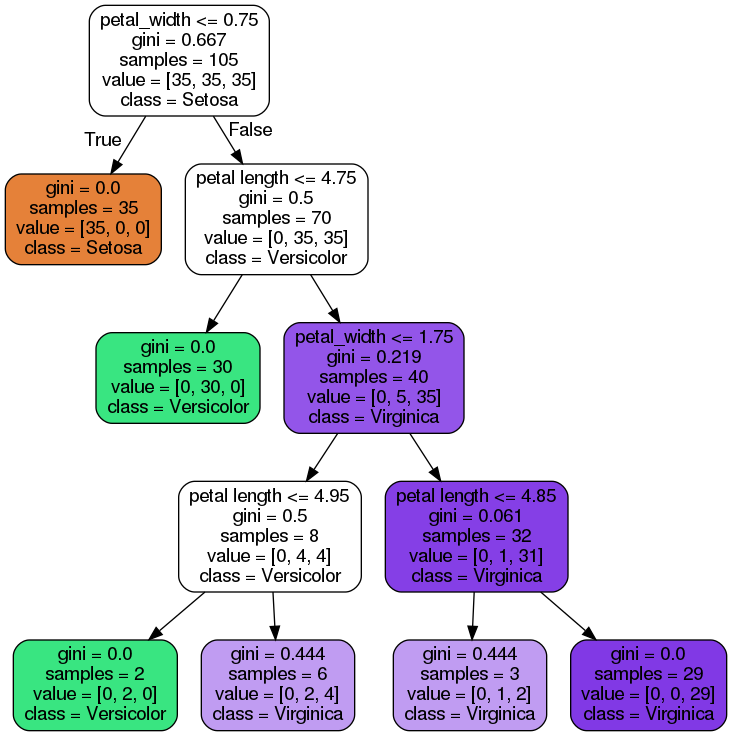
\includegraphics{tree.png}
\caption{tree-viz}
\end{figure}

    By using the \texttt{out\_file=None} setting, we directly assigned the
dot data to a \texttt{dot\_data} variable, instead of writing an
intermediate \texttt{tree.dot} file to disk. The arguments for
\texttt{filled}, \texttt{rounded}, \texttt{class\_names}, and
\texttt{feature\_names} are optional but make the resulting image file
visually more appealing by adding color, rounding the box edges, showing
the name of the majority class label at each node, and displaying the
feature names in the splitting criterion.

    \section{Random Forests}\label{random-forests}

Conveniently, we don't have to construct the random forest classifier
from the individual trees by ourselves because there is already an
implementation in scikit-learn that we can use. After executing the
preceding code, we should see the decision regions formed by the
ensemble of trees in the random forest, as shown in the upcoming figure.

    \begin{Verbatim}[commandchars=\\\{\}]
{\color{incolor}In [{\color{incolor}30}]:} \PY{k+kn}{from} \PY{n+nn}{sklearn}\PY{n+nn}{.}\PY{n+nn}{ensemble} \PY{k}{import} \PY{n}{RandomForestClassifier}
         
         \PY{n}{forest} \PY{o}{=} \PY{n}{RandomForestClassifier}\PY{p}{(}\PY{n}{criterion}\PY{o}{=}\PY{l+s+s1}{\PYZsq{}}\PY{l+s+s1}{gini}\PY{l+s+s1}{\PYZsq{}}\PY{p}{,}
                                         \PY{n}{n\PYZus{}estimators}\PY{o}{=}\PY{l+m+mi}{25}\PY{p}{,}
                                         \PY{n}{random\PYZus{}state}\PY{o}{=}\PY{l+m+mi}{1}\PY{p}{,}
                                         \PY{n}{n\PYZus{}jobs}\PY{o}{=}\PY{l+m+mi}{2}\PY{p}{)}
         
         \PY{c+c1}{\PYZsh{} The number of jobs to run in parallel for both fit and predict.}
         \PY{c+c1}{\PYZsh{} If \PYZhy{}1, then the number of jobs is set to the number of cores.}
         
         \PY{n}{forest}\PY{o}{.}\PY{n}{fit}\PY{p}{(}\PY{n}{X\PYZus{}train}\PY{p}{,} \PY{n}{y\PYZus{}train}\PY{p}{)}
         \PY{n}{plot\PYZus{}decision\PYZus{}regions}\PY{p}{(}\PY{n}{X\PYZus{}combined}\PY{p}{,} \PY{n}{y\PYZus{}combined}\PY{p}{,} \PY{n}{classifier}\PY{o}{=}\PY{n}{forest}\PY{p}{,} \PY{n}{test\PYZus{}idx}\PY{o}{=}\PY{n+nb}{range}\PY{p}{(}\PY{l+m+mi}{105}\PY{p}{,} \PY{l+m+mi}{150}\PY{p}{)}\PY{p}{)}
         \PY{n}{plt}\PY{o}{.}\PY{n}{xlabel}\PY{p}{(}\PY{l+s+s1}{\PYZsq{}}\PY{l+s+s1}{petal length [cm]}\PY{l+s+s1}{\PYZsq{}}\PY{p}{)}
         \PY{n}{plt}\PY{o}{.}\PY{n}{ylabel}\PY{p}{(}\PY{l+s+s1}{\PYZsq{}}\PY{l+s+s1}{petal width [cm]}\PY{l+s+s1}{\PYZsq{}}\PY{p}{)}
         \PY{n}{plt}\PY{o}{.}\PY{n}{legend}\PY{p}{(}\PY{n}{loc}\PY{o}{=}\PY{l+s+s1}{\PYZsq{}}\PY{l+s+s1}{upper left}\PY{l+s+s1}{\PYZsq{}}\PY{p}{)}
         \PY{n}{plt}\PY{o}{.}\PY{n}{show}\PY{p}{(}\PY{p}{)}
\end{Verbatim}


    \begin{center}
    \adjustimage{max size={0.9\linewidth}{0.9\paperheight}}{output_63_0.png}
    \end{center}
    { \hspace*{\fill} \\}
    
    Using the preceding code, we trained a random forest from 25 decision
trees via the \texttt{n\_estimators} parameter and used the gini
criterion as an impurity measure to split the nodes. Although we are
growing a very small forest from a very small training dataset, we used
the \texttt{n\_jobs} parameter for demonstration purposes, which allows
us to parallellize the model training using multiple cores or our
computer (in this particular example, 2 cores.)

    \section{K-nearest neighbors - a lazy learning
algorithm}\label{k-nearest-neighbors---a-lazy-learning-algorithm}

By executing the following code, we will now implement a KNN model in
scikit-learn using a Euclidean distance metric:

    \begin{Verbatim}[commandchars=\\\{\}]
{\color{incolor}In [{\color{incolor}31}]:} \PY{k+kn}{from} \PY{n+nn}{sklearn}\PY{n+nn}{.}\PY{n+nn}{neighbors} \PY{k}{import} \PY{n}{KNeighborsClassifier}
         
         \PY{n}{knn} \PY{o}{=} \PY{n}{KNeighborsClassifier}\PY{p}{(}\PY{n}{n\PYZus{}neighbors}\PY{o}{=}\PY{l+m+mi}{5}\PY{p}{,} \PY{n}{p}\PY{o}{=}\PY{l+m+mi}{2}\PY{p}{,} \PY{n}{metric}\PY{o}{=}\PY{l+s+s1}{\PYZsq{}}\PY{l+s+s1}{minkowski}\PY{l+s+s1}{\PYZsq{}}\PY{p}{)}
         \PY{n}{knn}\PY{o}{.}\PY{n}{fit}\PY{p}{(}\PY{n}{X\PYZus{}train\PYZus{}std}\PY{p}{,} \PY{n}{y\PYZus{}train}\PY{p}{)}
         
         \PY{n}{plot\PYZus{}decision\PYZus{}regions}\PY{p}{(}\PY{n}{X\PYZus{}combined\PYZus{}std}\PY{p}{,} \PY{n}{y\PYZus{}combined}\PY{p}{,} \PY{n}{classifier}\PY{o}{=}\PY{n}{knn}\PY{p}{,} \PY{n}{test\PYZus{}idx}\PY{o}{=}\PY{n+nb}{range}\PY{p}{(}\PY{l+m+mi}{105}\PY{p}{,} \PY{l+m+mi}{150}\PY{p}{)}\PY{p}{)}
         \PY{n}{plt}\PY{o}{.}\PY{n}{xlabel}\PY{p}{(}\PY{l+s+s1}{\PYZsq{}}\PY{l+s+s1}{petal length [standardised]}\PY{l+s+s1}{\PYZsq{}}\PY{p}{)}
         \PY{n}{plt}\PY{o}{.}\PY{n}{ylabel}\PY{p}{(}\PY{l+s+s1}{\PYZsq{}}\PY{l+s+s1}{petal width [standardised]}\PY{l+s+s1}{\PYZsq{}}\PY{p}{)}
         \PY{n}{plt}\PY{o}{.}\PY{n}{legend}\PY{p}{(}\PY{n}{loc}\PY{o}{=}\PY{l+s+s1}{\PYZsq{}}\PY{l+s+s1}{upper left}\PY{l+s+s1}{\PYZsq{}}\PY{p}{)}
         \PY{n}{plt}\PY{o}{.}\PY{n}{show}\PY{p}{(}\PY{p}{)}
\end{Verbatim}


    \begin{center}
    \adjustimage{max size={0.9\linewidth}{0.9\paperheight}}{output_66_0.png}
    \end{center}
    { \hspace*{\fill} \\}
    

    % Add a bibliography block to the postdoc
    
    
    
    \end{document}
